% This is samplepaper.tex, a sample chapter demonstrating the
% LLNCS macro package for Springer Computer Science proceedings;
% Version 2.21 of 2022/01/12
%
\documentclass[runningheads]{llncs}
%
\usepackage[T1]{fontenc}
\usepackage{amsmath}
\usepackage{booktabs}
\usepackage{multirow}
\usepackage{ulem}
\usepackage{graphicx}
\usepackage{adjustbox}
\usepackage{subcaption}
\usepackage{booktabs}  % For professional looking tables
\usepackage{array}     % To use column formatting
\usepackage{graphics}
% T1 fonts will be used to generate the final print and online PDFs,
% so please use T1 fonts in your manuscript whenever possible.
% Other font encondings may result in incorrect characters.
%
\usepackage{graphicx}
% Used for displaying a sample figure. If possible, figure files should
% be included in EPS format.
%
% If you use the hyperref package, please uncomment the following two lines
% to display URLs in blue roman font according to Springer's eBook style:
%\usepackage{color}
%\renewcommand\UrlFont{\color{blue}\rmfamily}
%\urlstyle{rm}
%
\begin{document}
%
\title{Large Language Models \\ for Logical Fallacy Detection}
%
%\titlerunning{Abbreviated paper title}
% If the paper title is too long for the running head, you can set
% an abbreviated paper title here
%

\author{Nicole Teo\inst{1}\orcidID{0009-0006-1497-2785} \and
Donghao Huang\inst{1,2}\orcidID{0009-0005-6767-4872} \and \\
Erik Cambria\inst{3}\orcidID{0000-0002-3030-1280} \and
Zhaoxia Wang\inst{1*}\orcidID{0000-0001-7674-5488}
}

\authorrunning{Teo et al.}
% First names are abbreviated in the running head.
% If there are more than two authors, 'et al.' is used.

% \institute{Singapore Management University, 80 Stamford Rd, Singapore 178902
% \email{nicolet.2023@engd.smu.edu.sg}\\
% \email{dh.huang.2023@engd.smu.edu.sg} \\
% \email{cambria@ntu.edu.sg} \\
% \email{zxwang@smu.edu.sg}\\
% }

\institute{Singapore Management University, 80 Stamford Rd, Singapore 178902 
\email{nicolet.2023@engd.smu.edu.sg, dh.huang.2023@engd.smu.edu.sg, zxwang@smu.edu.sg*}\\
\and Research and Development, Mastercard, 3 Fraser Street, Level 17, DUO Tower, Singapore 189352, Singapore \and
Nanyang Technological University, 50 Nanyang Ave, Singapore 639798
\email{cambria@ntu.edu.sg}}
%
\maketitle              % typeset the header of the contribution
%
\begin{abstract}
Identifying logical fallacies is essential for maintaining logical reasoning and reducing false information in a variety of domains, such as the media, law, and education. We present an extensive study on the use of large language models (LLMs) for logical fallacy detection and provide a comparative overview of model performance across various fallacy classes. We evaluate the logical fallacy detection capabilities of multiple state-of-the-art models (LLaMA, Qwen, Gemma, Phi) utilizing accuracy, precision, recall, and F1-score as assessment measures. According to our findings, our models do well on simple fallacies like ``circular reasoning,'' but they have trouble with more interpretive reasoning when it comes to more complex categories like ``equivocation'' and ``intentional''. These results highlight the potential of LLMs in fallacy detection tasks but also indicate a need for improved prompt engineering, fine-tuning, and context-rich datasets to enhance interpretive accuracy. This research offers insights into advancing LLMs for critical reasoning applications, contributing to improved information integrity across domains.

\keywords{Large language models  \and Logical fallacies \and Reasoning.}
\end{abstract}
%
%
%
\section{Background}
The rapid advancement of large language models (LLMs) has opened new avenues for natural language processing, allowing for exceptional performance on a variety of downstream tasks~\cite{jie2024self,grattafiori2024llama}. In addition, it has also expanded applications spanning from conversational agents to complex reasoning tasks~\cite{brown2020language,liu2024two,du2024evaluation}. Among these tasks, logical fallacy detection has emerged as a critical area of focus, given its implications for the integrity of information and reasoning processes in various domains, including education, law, and media literacy. Logical fallacies undermine sound argumentation and can lead to flawed conclusions, making the ability to identify and address these fallacies essential.

A fallacy is defined as ``a mistake in reasoning [...] that occurs with some frequency in real arguments and which is characteristically deceptive''~\cite{govier2018problems}. The task of classifying fallacies, or developing a classification model to distinguish between various forms of fallacies, has been taken up by recent publications~\cite{alhindi2023multitask}.~\cite{jin2022logical} combined methods like large transformer language models and the Structure Aware Hypothesis~\cite{yin2019benchmarking} from natural language inference. In this line of study, the underlying logical shape of the text is extracted via argument mining~\cite{lawrence2020argument}, and the resulting features are used to train a classifier. Interestingly, the datasets presented by~\cite{jin2022logical} only include false assertions, which means that they may only be classified as fallacious types if the argument is presumed to be false. More recently,~\cite{lim2024evaluation} focused on assessing the effectiveness of GPT-4, in identifying logical fallacies as part of a digital misinformation intervention. This evaluation is particularly important because logical fallacies are a common feature in misinformation, and understanding the capabilities of LLMs in this domain could aid in combating such content. They found that while GPT-4 showed strong performance in identifying logical fallacies, its performance varied across different types of fallacies. 

This study investigates the ability of leading LLMs—LLaMA, Qwen, Gemma, and Phi—to detect logical fallacies using metrics like accuracy, F1-score, recall, and precision. We also analyze their sensitivity to different fallacy types to better understand their reasoning processes. To enhance interpretability, we apply methods from interpretable AI, offering insights into model decisions and increasing transparency and accountability. By providing justifications for classifications, we aim to clarify how LLMs identify fallacies and support their use in fostering critical thinking and informed decision-making.

% In this study, we conduct an extensive investigation into the capabilities of several state-of-the-art LLMs—specifically LLaMA, Qwen, Gemma, and Phi—in detecting logical fallacies. We employ a comprehensive set of evaluation metrics, including accuracy, F1-score, recall, and precision, to assess their performance and identify strengths and weaknesses in their detection capabilities. Additionally, our research examines the sensitivity of these models to different types of logical fallacies, offering insights into their reasoning processes.

% Recognizing the importance of interpretability in artificial intelligence (AI), we integrate approaches from  interpretable AI to enhance our findings. This focus on transparency not only aids in understanding model decision-making processes but also strengthens the accountability and reliability of LLMs in logical reasoning tasks. By providing justifications for model classifications, we aim to demystify the reasoning behind the detection of logical fallacies. Through this work, we aspire to contribute to a deeper understanding of LLMs and their potential applications in promoting critical thinking and informed decision-making.

% Recognizing the importance of explainability in artificial intelligence, we integrate approaches from explainable AI (XAI) to enhance the interpretability of our findings. This focus on transparency not only aids in understanding model decision-making processes but also strengthens the accountability and reliability of LLMs in logical reasoning tasks. By providing justifications for model classifications, we aim to demystify the reasoning behind the detection of logical fallacies. Ultimately, this research serves as a foundation for future developments in error detection and model explainability, paving the way for more transparent and efficient AI systems capable of engaging in logical reasoning. Through this work, we aspire to contribute to a deeper understanding of LLMs and their potential applications in promoting critical thinking and informed decision-making.

Our work aims to present a thorough analysis across different LLMs for the identification of logical fallacies, together with new methods for evaluating the interpretability and effectiveness of these models. The primary contributions we have made in this paper are:
\begin{enumerate}
    %\item A comprehensive evaluation of LLMs, such as LLaMA, Qwen, Gemma, and Phi, with a focus on their performance in detecting logical fallacies in textual data.
   % \item A comparative overview of model performance across various fallacy classes. 
   \item The paper presents a comprehensive analysis of state-of-the-art LLMs (LLaMA, Qwen, Gemma, Phi) for detecting various types of logical fallacies, providing insights into their strengths and weaknesses.
   \item The study highlights how LLMs perform differently across fallacy categories, showing strong results on simpler fallacies like ``circular reasoning'' while facing challenges with more complex types such as ``equivocation'' and ``intentional.''
   \item The research suggests enhancements in prompt engineering, fine-tuning, and dataset design, offering practical guidance for improving LLMs' ability to detect and interpret complex logical fallacies.
   
\end{enumerate}

\section{Related Work}

\textbf{Logical Reasoning}. Recent developments have demonstrated that LLMs may generate intermediate reasoning stages to carry out reasoning tasks efficiently~\cite{shen2025reasoning,wang2024reasoning,yang2022language}. Formal reasoning, which is frequently applied in logic and mathematics, is a methodical, logical process that adheres to a set of norms and principles. Informal reasoning, which is more prevalent in daily life, is a less formal method of problem solving that depends on experience, common sense, and intuition to reach conclusions. Informal reasoning is more flexible and open-ended but may also be less reliable than formal reasoning, which is more ordered and dependable~\cite{huang2022towards}. The logical reasoning skills of large language models are gaining more and more attention from researchers~\cite{huang2025logical,xu2025large,zhou2022least,parmar2024logicbench}. 
%sanyal2022apollo
For example,~\cite{olausson2023linc} integrated first-order logic with large language models.~\cite{pan2023logic} and~\cite{zhang2023improved} equipped extensive language models with symbolic solutions. An adversarial pre-training approach was presented by~\cite{pi2022logigan} to improve logical thinking. Multi-step explicit planning was added to the inference process by~\cite{zhang2023improved}.
A contrastive learning strategy was put up by~\cite{jiao2022merit} to enhance logical question responding. 

\textbf{Logical Fallacies}. False reasoning patterns are known as logical fallacies~\cite{fantino2003logical}. They are frequently recognized since their claims are not backed up by any proof. Finding logical fallacies in natural language text has a wide range of possible uses, including tracking false information and confirming assertions. Furthermore, being able to understand erroneous arguments can improve the logic and educational value of speech. Fallacies can also be deliberately committed in order to mislead or influence others, and have been used to disseminate propaganda in news articles~\cite{musi2022developing}. Recent attempts have been made to categorize fallacies using deep learning models. For example~\cite{jin2022logical} proposed a dataset, where the fallacies were categorized using a structure-based approach. Follow up work has also tried to classify logical fallacies and valid statements~\cite{lalwaniexplainnli}, and build a software that addresses question-answering fallacies~\cite{habernal2017argotario}.~\cite{sheng2020nice} investigated discussion answers for the ad hominem fallacy. In their study,~\cite{habernal2018before} investigated the ad hominem fallacy in online arguments. Argumentation essays were found to have weak arguments by~\cite{stab2017recognizing}. A multi-task prompting technique was presented by~\cite{alhindi2023multitask}. It allows users to collaboratively learn fallacies from several datasets. To our knowledge, no prior work has tried to test out the logical fallacy detection capabilities of recent open source LLMs.  

\section{Methodology}
In this study, we evaluate the logical fallacy detection capabilities of different state-of-the-art large language models, such as LLaMA, Qwen, Gemma, and Phi. These models were selected based on their recent advancements in natural language understanding and generation, as well as their potential to address complex reasoning tasks such as logical fallacy detection. Each model was evaluated in the context of its ability to identify fallacies across a range of types, including simple and complex categories.

%This section also outlines the metrics and evaluation data, the baselines we use for comparison, and the specifics of the implementation.
This section also outlines the data used for evaluation, data pre-processing, evaluation and implementation,  the baselines for comparison, and the specifics of the implementation.

\subsection{Dataset}
We make use of the LOGIC and LOGIC Climate logical fallacy datasets from~\cite{jin2022logical}, which has 2,449 instances of logical fallacies spanning 13 different categories. The LOGIC dataset comprises of typical instances of logical fallacies gathered from several online educational resources designed to instruct or assess students' comprehension of logical fallacies. The logical fallacy examples was gathered manually from Google, totaling about 600 samples, and automatically gathered from three student quiz websites: Quizziz, study.com, and ProProfs~\cite{jin2022logical}. The LOGIC Climate dataset contains more difficult examples of the same logical error types on the subject of climate change. It comprises of 1,079 samples of logical fallacies, with an average of 35.98 tokens per sample and a vocabulary of 5.8K words. 
%We use the standard metrics of weighted precision, recall, and F1-score and model the classification task as a classification issue. 
A sample of the dataset structure is illustrated in Table~\ref{tab:logicstructure}. The full dataset contains 13 logical fallacy types, each represented by exemplar statements that demonstrate the reasoning error characteristic of that fallacy category.

\begin{table}[h!]
    \centering
    \caption{Structure of the LOGIC Dataset}
    \label{tab:logicstructure}
    \begin{tabular}{|p{9.2cm}|p{3.1cm}|}
        \hline
        \textbf{Text} & \textbf{Label} \\
        \hline
        ``You're too ugly to be class president!'' & Ad Hominem \\
        Everyone is going to get the new smart phone when it comes out this weekend. Why aren't you? & Ad Populum \\
        Do the best for your baby & Appeal to Emotion \\
        America is the best place to live, because it's better than any other country. & Circular Reasoning \\
        Noisy children are a real headache. Two aspirin will make a headache go away. Therefore, two aspirin will make noisy children go away. & Equivocation \\
        I am committed to preserving traditional marriage, the union of one man and one woman. & Fallacy of Credibility \\
        The Senator thinks we can solve all our ecological problems by driving a Prius. & Fallacy of Extension \\
        Most Arabs are Muslims and all the 9/11 hijackers were also Muslims. Therefore most Arabs are hijackers. & Fallacy of Logic \\
        ``I believe deeply that canceling the fashion show is the best decision. I know it is. I am very certain about it.'' & Fallacy of Relevance \\
        The Soviet Union collapsed after taking up atheism. Therefore, we must avoid atheism for the same reasons. & False Causality \\
        You need to go to the party with me, otherwise you'll just be bored at home. & False Dilemma \\
        If we let this child bring the permission slip late, there is no reason to ever set a deadline for anything again! & Faulty Generalization \\
        You can't prove that space aliens don't exist, so they must be real & Intentional \\
        \hline
    \end{tabular}
\end{table}

% \begin{table}[h!]
%     \centering
%     \caption{Structure of the LOGIC Dataset}
%     \label{tab:logicstructure}
%     \begin{tabular}{|p{9cm}|p{3cm}|}
%         \hline
%         \textbf{Text} & \textbf{Label} \\
%         \hline
%         You need to go to the party with me, otherwise, you'll regret it. & False Dilemma \\
%         If we let this child bring the permission slip late, soon everyone will want to. & Faulty Generalization \\
%         I am committed to preserving traditional marriage because that’s how it has always been. & Fallacy of Credibility \\
%         ``I believe deeply that canceling the fashion show is wrong because it just feels unfair.'' & Fallacy of Relevance \\
%         Most Arabs are Muslims and all the 9/11 hijackers were Arab; therefore, all Muslims are terrorists. & Fallacy of Logic \\
%         \hline
%     \end{tabular}
% \end{table}

% \begin{table}[h!]
%     \centering
%     \caption{Structure of the LOGIC Climate Dataset}
%     \label{tab:logicclimatestructure}
%     \begin{tabular}{|p{10cm}|p{4cm}|}
%         \hline
%         \textbf{Text} & \textbf{Label} \\
%         \hline
%         Rep. Bill Posey (R-FL) said scientists said ... & Intentional \\
%         ``Look, if you want to characterize a temper... & Intentional \\
%         At one point, Smith showed a slide of two ch... & Intentional \\
%         Brooks then said that erosion plays a significant role... & Faulty Generalization \\
%         Brooks added that Antarctic ice is growing. & Intentional \\
%         \hline
%     \end{tabular}
% \end{table}

\subsection{Data Pre-processing}
Each dataset contained text samples with corresponding issue labels. We began by filtering out rows with missing values to ensure consistency and avoid performance issues during modeling. Next, we applied label encoding to convert categorical labels into numerical form, standardizing the format for both datasets.

To prepare the text for model training, we used TF-IDF vectorization with a maximum of 5000 features, capturing the most informative terms while reducing computational load and overfitting. The vectorizer was fitted on the training data and then applied to the test set to maintain a consistent feature space. Finally, we split the training data into 80\% for training and 20\% for validation.

% Each dataset included a series of text samples that described different issues along with the labels that went with them. In order to preserve only the relevant columns, we first filtered these datasets, eliminating any rows that had missing values in any of these columns. By removing null values from the datasets, this data cleaning stage made sure they were consistent and would not affect model performance or downstream processing. After cleaning, we converted the categorical labels in the label column into numerical representations by applying label encoding. By standardizing the label format for both datasets, this step allowed the machine learning model to understand them consistently. 

% For model training, we used Term Frequency-Inverse Document Frequency (TF-IDF) vectorization to transform the text input into a numerical format. The text data was successfully converted into a vector space model based on the relative relevance of terms across publications with a maximum feature limit of 5000. By concentrating on the most informative terms in the corpus, this feature restriction assisted in lowering computational demands and mitigating overfitting. To preserve a consistent feature space across the two sets, we first fitted the vectorizer to the training data and then used the fitted model to transform the testing data. In order to generate a validation set from the training data, we lastly incorporated a data-splitting step. We separated the data using an 80-20 split, setting aside 20\% of the training data as a validation set. 

\subsection{Implementation and Evaluation} %LLMs performance}

\textbf{Baseline}. We began by loading a tokenizer and a pre-trained LLM for sequence classification, adjusting the label size to match our dataset classes. The token embeddings were resized to fit the tokenizer's vocabulary, and the end-of-sequence token was set as the padding token to ensure consistent tokenization. Each sample was tokenized to a uniform length of 512 tokens with padding as needed, enabling efficient batching during training. We monitored precision, recall, and F1-score to track performance. Training used a learning rate of 2e-5 over 5 epochs, with weight decay (0.01) and a linear learning rate scheduler for regularization.

% We started by loading a tokenizer and a previously trained model. For sequence classification, the open source LLM model was set up with a label size that corresponded to the various classes in our dataset. To enable the model to process the whole token range, we expanded the token embeddings to match the tokenizer's vocabulary size. To guarantee uniform tokenization across samples, we designated the tokenizer's end-of-sequence token as the padding token as it did not initially have one. Each sample is then tokenzied in order to prepare the text data for the model. We made sure that the length of each token was uniform by setting to 512 tokens and using padding as needed. During training, this dataset format made batching effective and scalable. The metrics tracked are precision, recall, and F1-score, in order to efficiently monitor model performance. We set a learning rate of 2e-5, and 5 epochs. For better regularization, a weight decay of 0.01 and a linear learning rate scheduler were also added. 

\textbf{Few-shot}. We applied a few-shot learning approach by embedding three relevant text-label examples from the training data into each prompt. This format provides contextual guidance, helping the model predict labels for new inputs based on similar cases. These few-shot prompts are tokenized efficiently, ensuring they stay within model limits for smooth batch processing. Each dataset instance includes the tokenized prompt and label tensor, supporting training and evaluation. By integrating context directly into inputs, this method aims to boost model accuracy on unseen data.

% We used a few-shot learning approach to classify text inputs by embedding relevant examples directly into the prompts. By creating prompts with instances of text-label combinations taken from the training data, the few-shot learning component is controlled. These prompts are constructed to append a few (three in this case) sample text-label pairs to each input. The model receives contextual assistance from this format, which helps it anticipate labels for the new text input by providing it with information about related examples. Similar labeled instances are included directly in the prompt, giving the model additional context and possibly enhancing its performance on unseen data. These few-shot instructions are incorporated into tokenization. By ensuring that every input sequence falls inside the tokenization bounds of the model, this phase enables effective batch processing without consuming an excessive amount of memory. Each dataset instance is created with the tokenized few-shot prompts and label tensors, facilitating data feeding during training and evaluation. By adding relevant contextual examples to each input, this few-shot technique, which is directly incorporated into the training and evaluation pipeline, aims to increase model accuracy.

%\subsection{Model performance evaluation in different fallacy classes}
\textbf{Model performance evaluation in different fallacy classes.}
We generate a confusion matrix that visualizes the performance of a classification model. First, predictions are obtained from the model on the validation dataset. The predicted labels are extracted by selecting the highest probability class from the model's predictions, and the true labels are also collected. The confusion matrix, which compares the true labels with the predicted labels, is then computed. A custom function is then defined to plot the matrix as a heatmap with annotations, where the x-axis represents predicted labels, and the y-axis represents true labels. Finally, the function is called with class names (obtained from the label encoder) and the matrix is saved.

\section{Results}

\begin{table}[!ht]
\caption{Comparison of the best results of baseline (zero-shot) and few-shot prompting on LOGIC and LOGIC Climate. The best results per model are \textbf{boldfaced} and the overall best results are \underline{underlined}.}
\label{tab:performance}
\centering
\renewcommand{\arraystretch}{1.0} % Row height
\setlength{\tabcolsep}{5pt} % Column spacing
\begin{adjustbox}{max width=\textwidth}
\begin{tabular}{llcccccccc}
\toprule
\multirow{2}{*}{\textbf{Model}} & \multirow{2}{*}{\textbf{Type}} & \multicolumn{4}{c}{\textbf{LOGIC}} & \multicolumn{4}{c}{\textbf{LOGIC Climate}} \\
\cmidrule(lr){3-6} \cmidrule(lr){7-10}
& & \textbf{A} & \textbf{P} & \textbf{R} & \textbf{F1} & \textbf{A} & \textbf{P} & \textbf{R} & \textbf{F1} \\
\midrule
\multirow{2}{*}{Llama-3.2-1B-Instruct} & baseline & 0.562 & 0.578 & 0.562 & 0.562 & 0.232 & \textbf{0.276} & 0.232 & 0.214 \\
& few-shot & \textbf{0.631} & \textbf{0.646} & \textbf{0.631} & \textbf{0.632} & \textbf{0.261} & 0.225 & \textbf{0.261} & \textbf{0.226} \\
\midrule
\multirow{2}{*}{Llama-3.2-3B-Instruct} & baseline & 0.595 & 0.616 & 0.595 & 0.592 & 0.213 & 0.207 & 0.213 & 0.191 \\
& few-shot & \textbf{0.704} & \underline{\textbf{0.724}} & \textbf{0.704} & \textbf{0.698} & \textbf{0.237} & \textbf{0.323} & \textbf{0.237} & \textbf{0.210} \\
\midrule
\multirow{2}{*}{Qwen2.5-1.5B-Instruct} & baseline & 0.613 & 0.631 & 0.613 & 0.614 & 0.251 & 0.230 & 0.251 & 0.232 \\
& few-shot & \textbf{0.628} & \textbf{0.690} & \textbf{0.628} & \textbf{0.636} & \textbf{0.265} & \textbf{0.297} & \textbf{0.265} & \textbf{0.247} \\
\midrule
\multirow{2}{*}{Qwen2.5-3B-Instruct} & baseline & 0.601 & 0.627 & 0.601 & 0.600 & 0.227 & \textbf{0.263} & 0.227 & \textbf{0.227} \\
& few-shot & \textbf{0.680} & \textbf{0.712} & \textbf{0.680} & \textbf{0.682} & \textbf{0.242} & 0.260 & \textbf{0.242} & 0.217 \\
\midrule
\multirow{2}{*}{Gemma-7b-it} & baseline & 0.544 & \textbf{0.648} & 0.544 & \textbf{0.551} & 0.171 & \textbf{0.261} & 0.171 & \textbf{0.137} \\
& few-shot & \textbf{0.550} & 0.545 & \textbf{0.550} & 0.543 & \textbf{0.190} & 0.126 & \textbf{0.190} & 0.125 \\
\midrule
\multirow{2}{*}{Gemma-2-2b-it} & baseline & 0.595 & 0.602 & 0.595 & 0.587 & 0.246 & 0.267 & 0.246 & 0.222 \\
& few-shot & \textbf{0.674} & \textbf{0.681} & \textbf{0.674} & \textbf{0.669} & \textbf{0.294} & \underline{\textbf{0.366}} & \textbf{0.294} & \textbf{0.269} \\
\midrule
\multirow{2}{*}{Phi-3-mini-4k-instruct} & baseline & 0.637 & 0.665 & 0.637 & 0.642 & 0.237 & 0.238 & 0.237 & 0.216 \\
& few-shot & \textbf{0.695} & \textbf{0.712} & \textbf{0.695} & \textbf{0.690} & \textbf{0.322} & \textbf{0.323} & \textbf{0.322} & \underline{\textbf{0.297}} \\
\midrule
\multirow{2}{*}{Phi-3.5-mini-instruct} & baseline & 0.640 & 0.682 & 0.640 & 0.647 & 0.251 & 0.206 & 0.251 & 0.222 \\
& few-shot & \underline{\textbf{0.713}} & \textbf{0.721} & \underline{\textbf{0.713}} & \underline{\textbf{0.708}} & \underline{\textbf{0.332}} & \textbf{0.293} & \underline{\textbf{0.332}} & \textbf{0.292} \\
\bottomrule
\end{tabular}
\end{adjustbox}
\end{table}

Table \ref{tab:performance} presents a comparative analysis of baseline (zero-shot) and few-shot prompting across various models on the LOGIC and LOGIC Climate datasets. Accuracy (A), precision (P), recall (R), and F1-score (F1) are among the measures that are assessed. The findings show that few-shot prompting clearly outperforms zero-shot prompting for all models, with notable gains in accuracy and F1-score. The few-shot method shows significant improvements in predicting accuracy and improves the algorithms' capacity to categorize logical fallacies.

Phi-3.5-mini-instruct (few-shot) achieves the highest F1-score (0.708) and accuracy (0.713) on the LOGIC dataset, making it the best-performing model. Llama-3.2-3B-Instruct (few-shot) leads in precision (0.724) and recall (0.704). Other models, like Gemma-2-2b-it (few-shot) and Phi-3-mini-4k-instruct, also perform well with F1-scores above 0.690. Larger models generally outperform baselines and benefit most from few-shot prompting. LOGIC Climate proves more challenging, with lower scores across models. Gemma-2-2b-it (few-shot) ranks highest with 0.332 accuracy and 0.269 F1-score, followed by Phi-3-mini-4k-instruct (few-shot) at 0.322 accuracy and 0.297 F1-score. The results highlight the need for further fine-tuning and dataset-specific adjustments.

There are a number of reasons why certain networks perform poorly on the LOGIC Climate dataset in comparison to the standard LOGIC dataset. There are knowledge gaps since many LLMs are not expressly trained on climate-related talks, which frequently require domain-specific knowledge, scientific terminology, and politically sensitive disputes. It is more challenging to classify logical fallacies in climate discourse since they are typically more nuanced and include cherry-picking evidence, misinterpreting scientific uncertainties, and emotionally laden arguments. The notably poorer accuracy, precision, recall, and F1-scores for all models point to a basic difficulty in spotting fallacies in arguments pertaining to climate change. Although performance is enhanced by few-shot learning, the benefits are not significant, indicating that adaptive learning is insufficient to make up for domain knowledge deficiencies. While some models, like LLaMA-3.2-1B/3B and Gemma-7B/2B, struggle more, suggesting a lack of adaptation to domain-specific logical reasoning, others, like Phi-3.5-mini-instruct and Phi-3-mini-4k-instruct, do better, probably because they can follow instructions.

% When comparing the various model families, it can be shown that the Llama models fare well in LOGIC but not so well in LOGIC Climate. With few-shot prompting, the Qwen models exhibit a consistent improvement, especially Qwen2.5-1.5B, which obtains an F1-score of 0.636 in LOGIC. In LOGIC Climate, Gemma models—particularly Gemma-2-2b-it (few-shot)—perform remarkably well, while in LOGIC, they lag somewhat behind Phi models. Notably, the Phi models are excellent candidates for logical fallacy identification, especially Phi-3.5-mini-instruct and Phi-3-mini-4k-instruct, which routinely rate among the top. The findings demonstrated that few-shot prompting improves classification performance considerably, frequently resulting in an F1-score improvement of 10-15\% over zero-shot prompting. This pattern emphasizes how crucial it is to give models a limited quantity of labeled samples in order to enhance generalization. The distinctions between LOGIC and LOGIC Climate show that, even with the most advanced models, logical error identification is still difficult in more complex or domain-specific situations.

\begin{figure*}[!ht]
    \centering
    \begin{subfigure}[b]{0.45\textwidth}
        \centering
        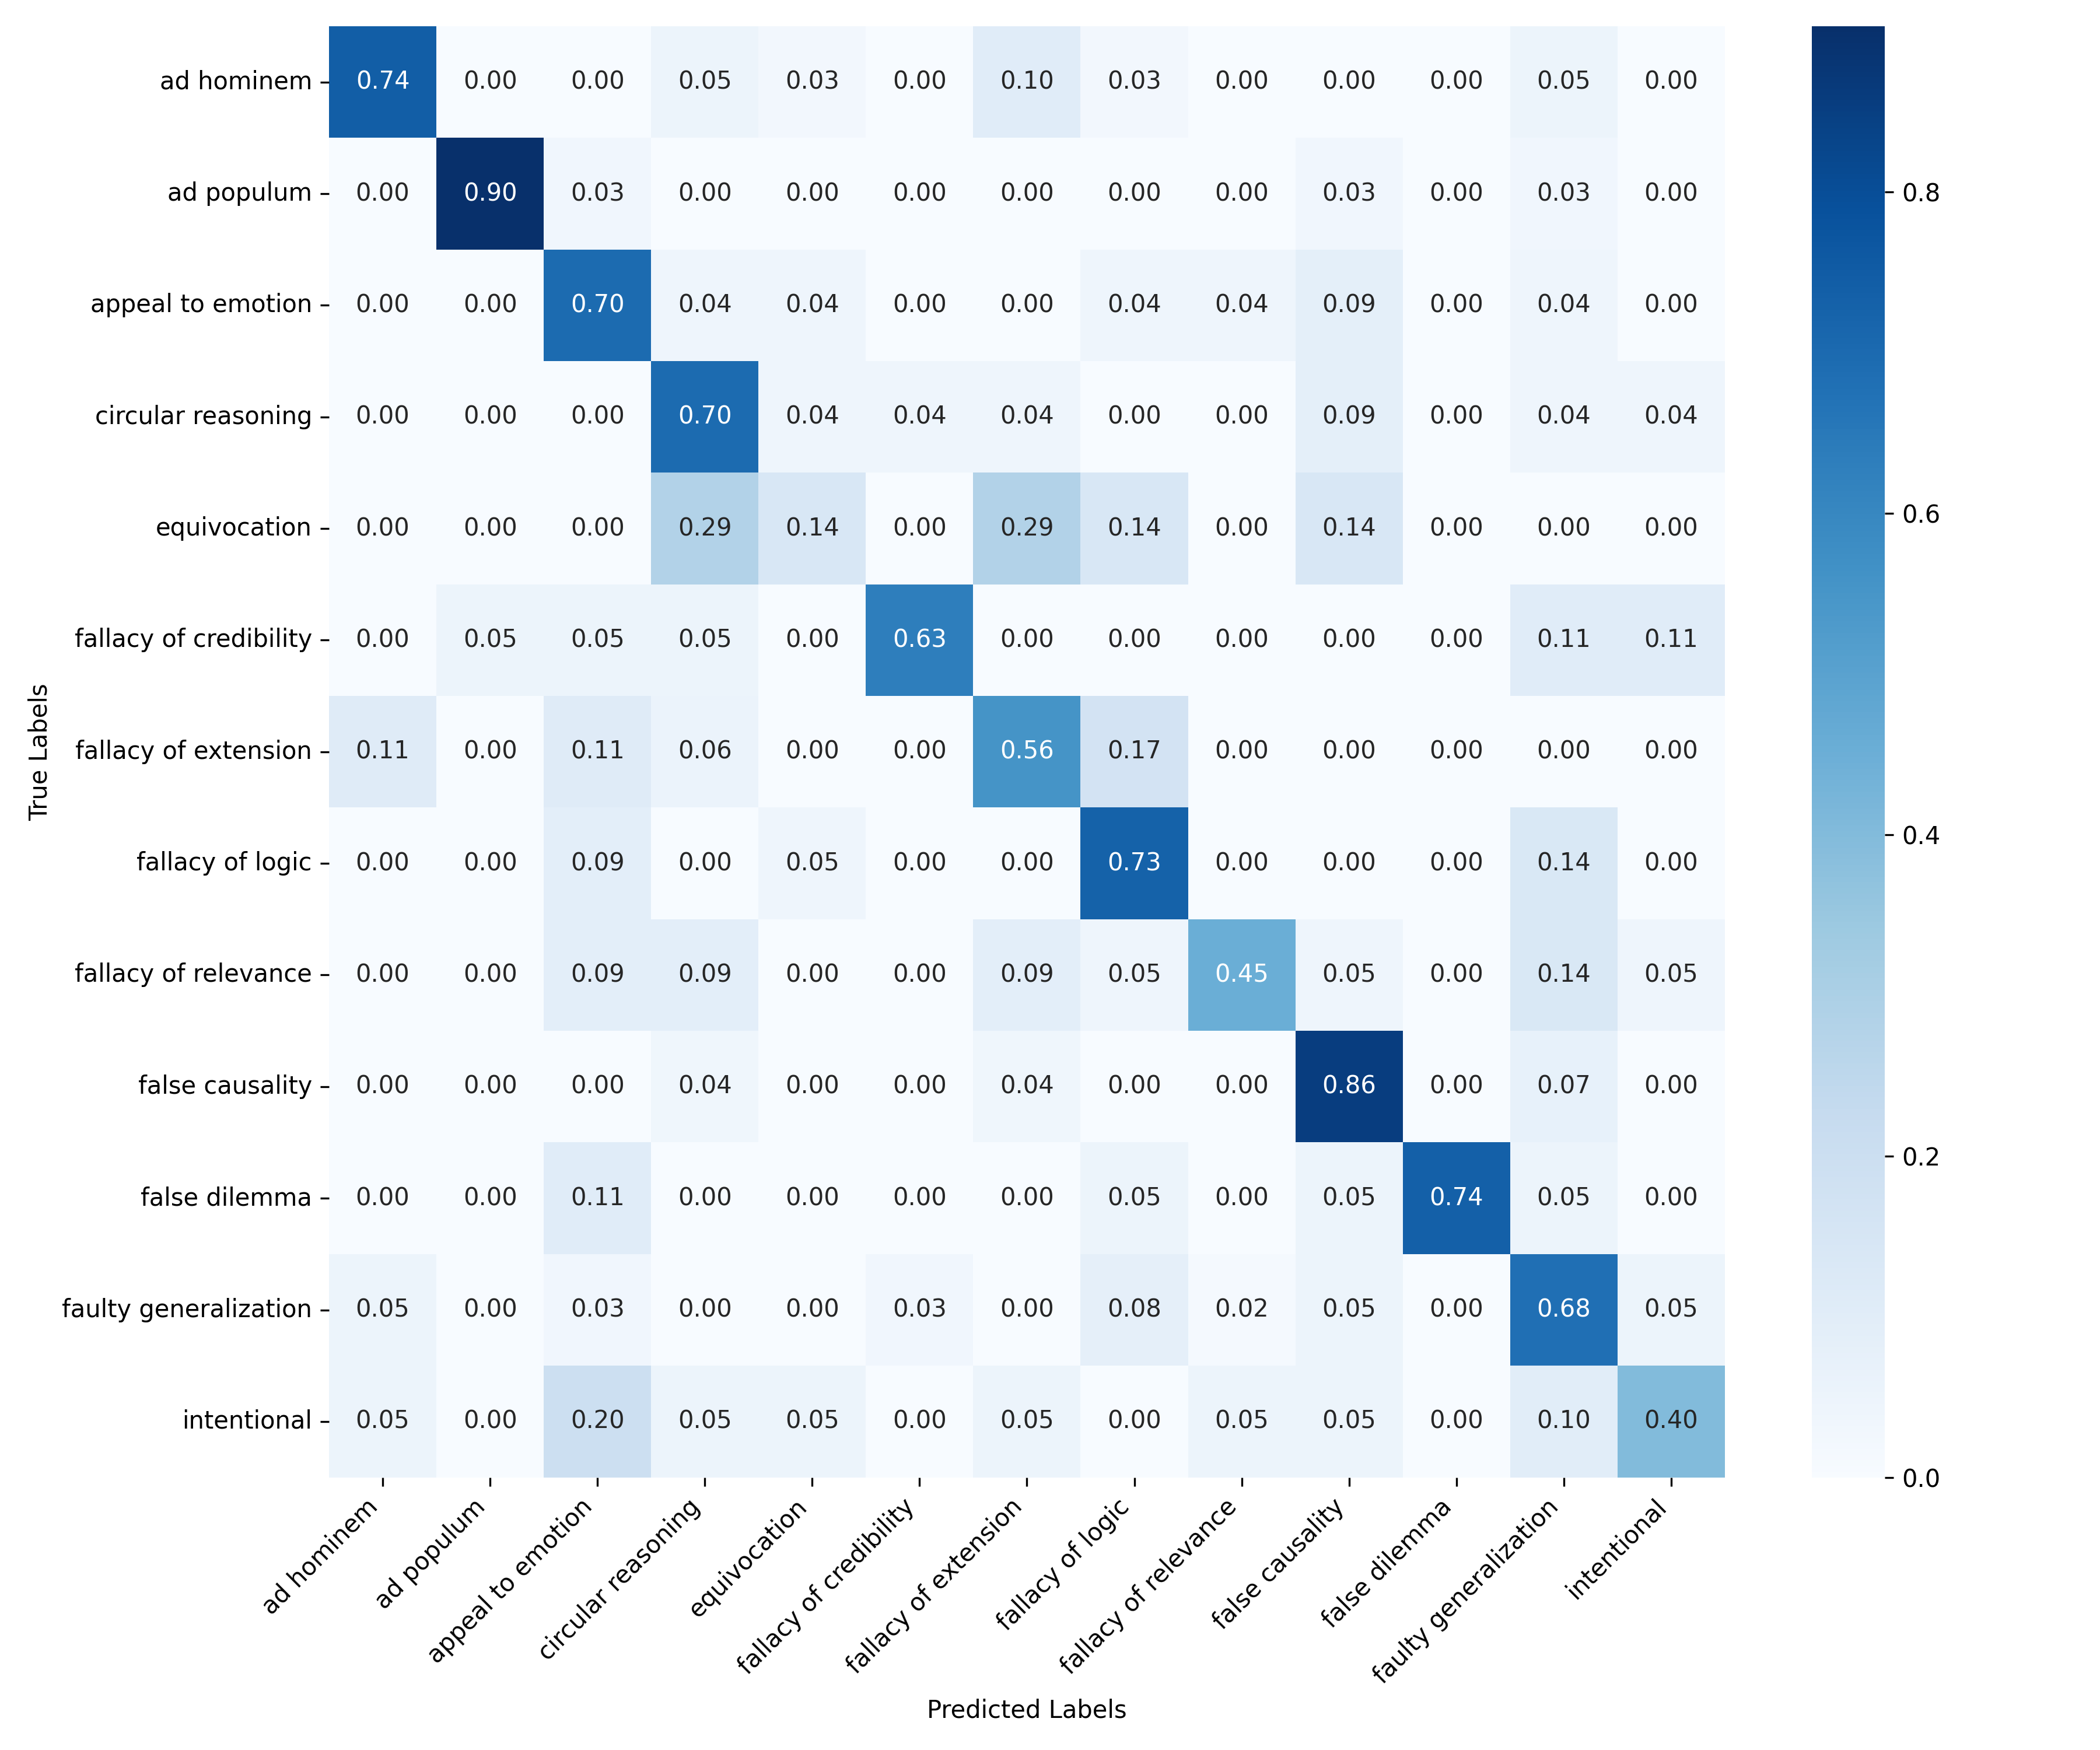
\includegraphics[width=\textwidth]{images/llama_logic_matrix.png}
        \caption{Llama-3.2-3B-Instruct}
        \label{fig:llama_confusion}
    \end{subfigure}
    \hfill
    \begin{subfigure}[b]{0.45\textwidth}
        \centering
        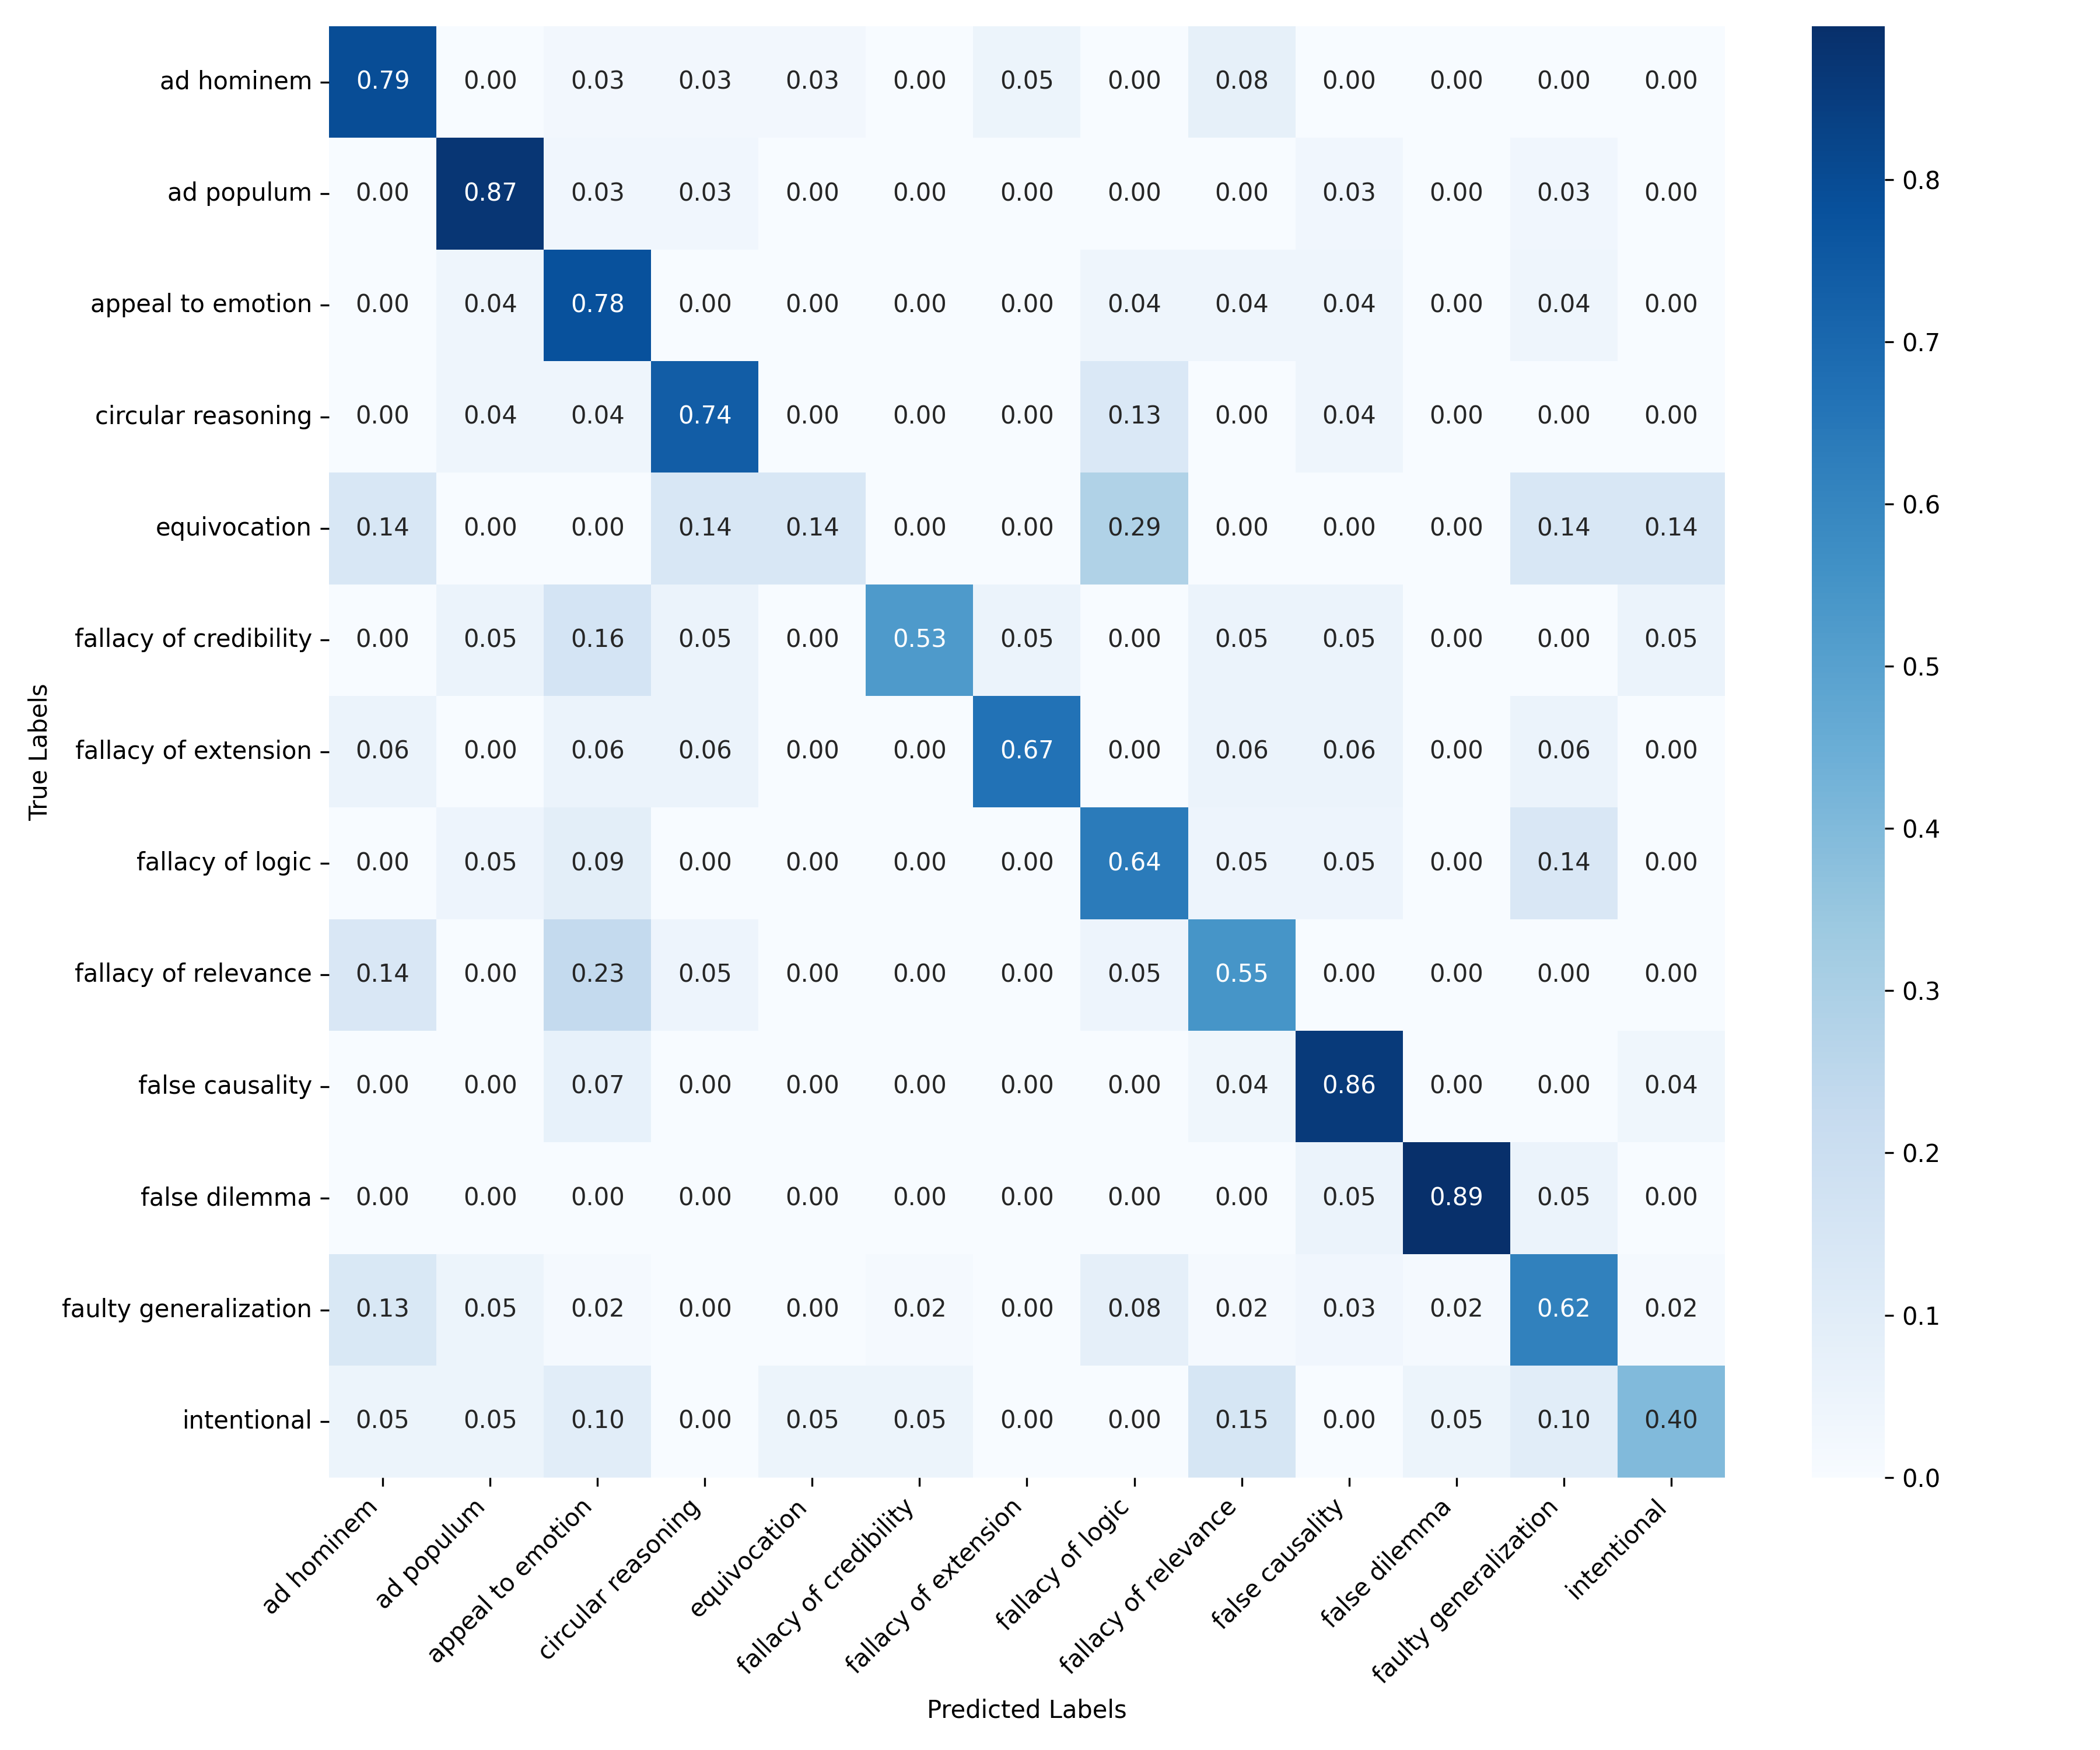
\includegraphics[width=\textwidth]{images/qwen_logic_matrix.png}
        \caption{Qwen2.5-3B-Instruct}
        \label{fig:qwen_confusion}
    \end{subfigure}
    \vskip\baselineskip
    \begin{subfigure}[b]{0.45\textwidth}
        \centering
        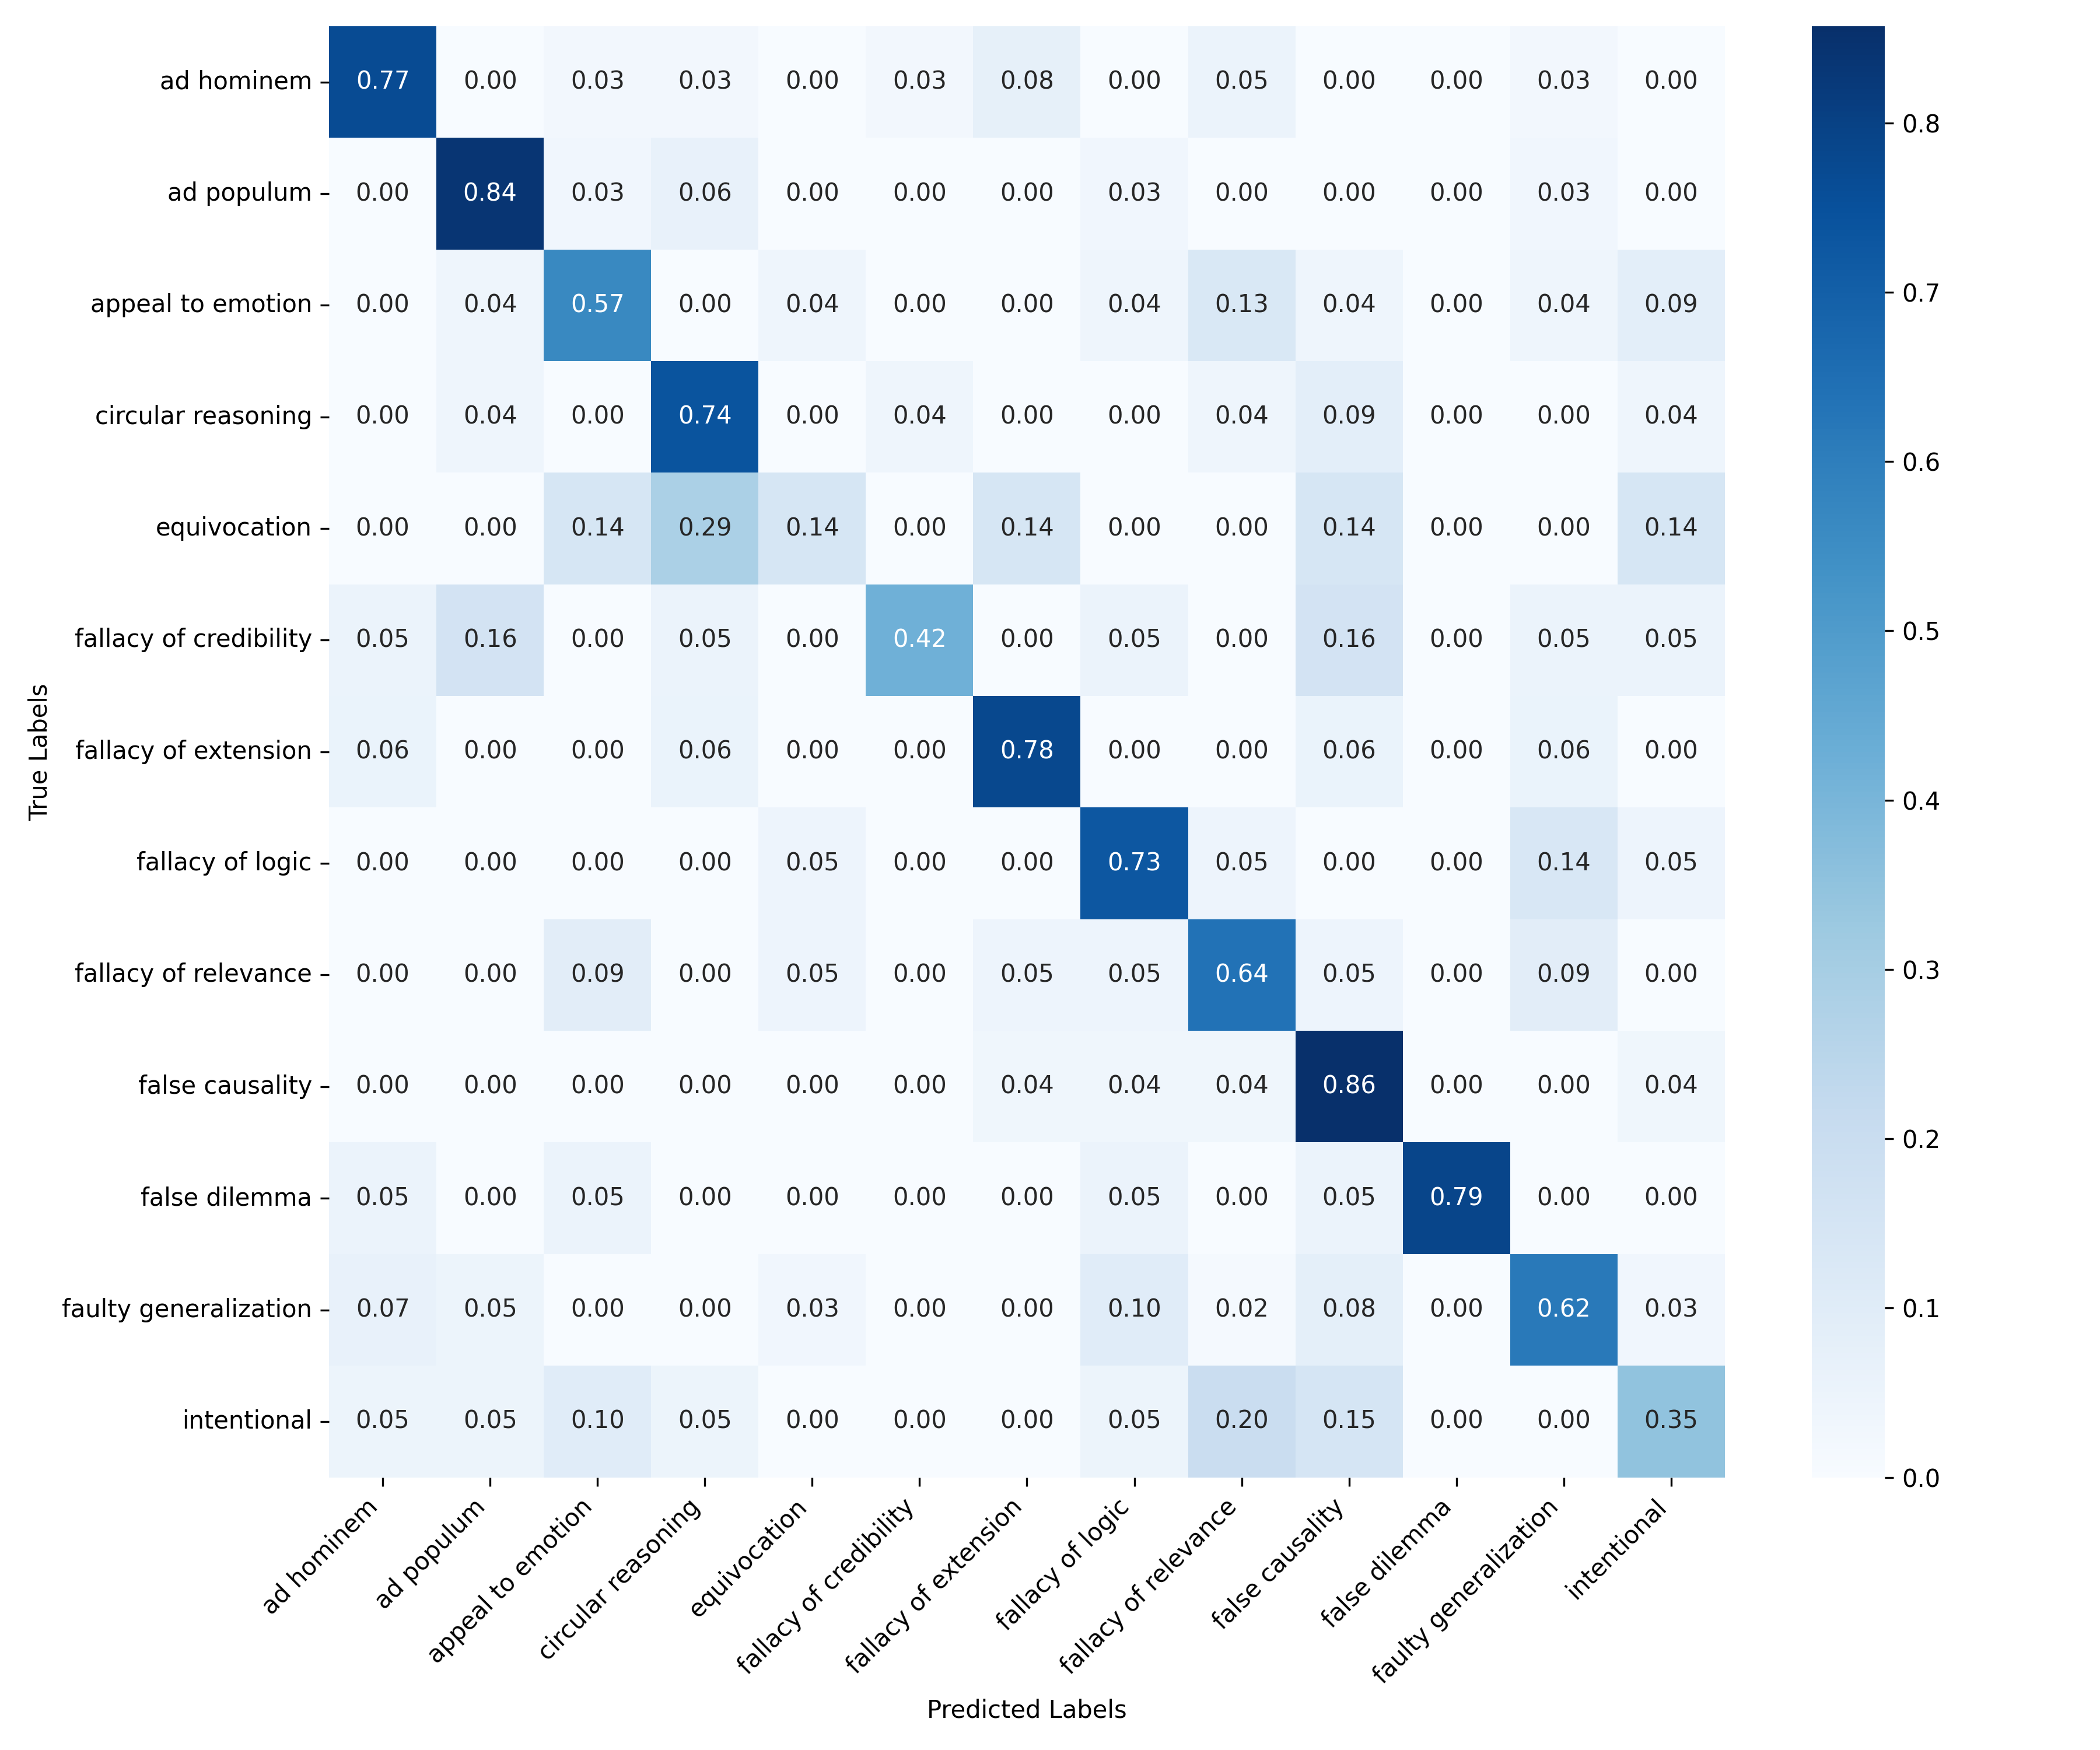
\includegraphics[width=\textwidth]{images/gemma_logic_matrix.png}
        \caption{Gemma-2-2b-it}
        \label{fig:gemma_confusion}
    \end{subfigure}
    \hfill
    \begin{subfigure}[b]{0.45\textwidth}
        \centering
        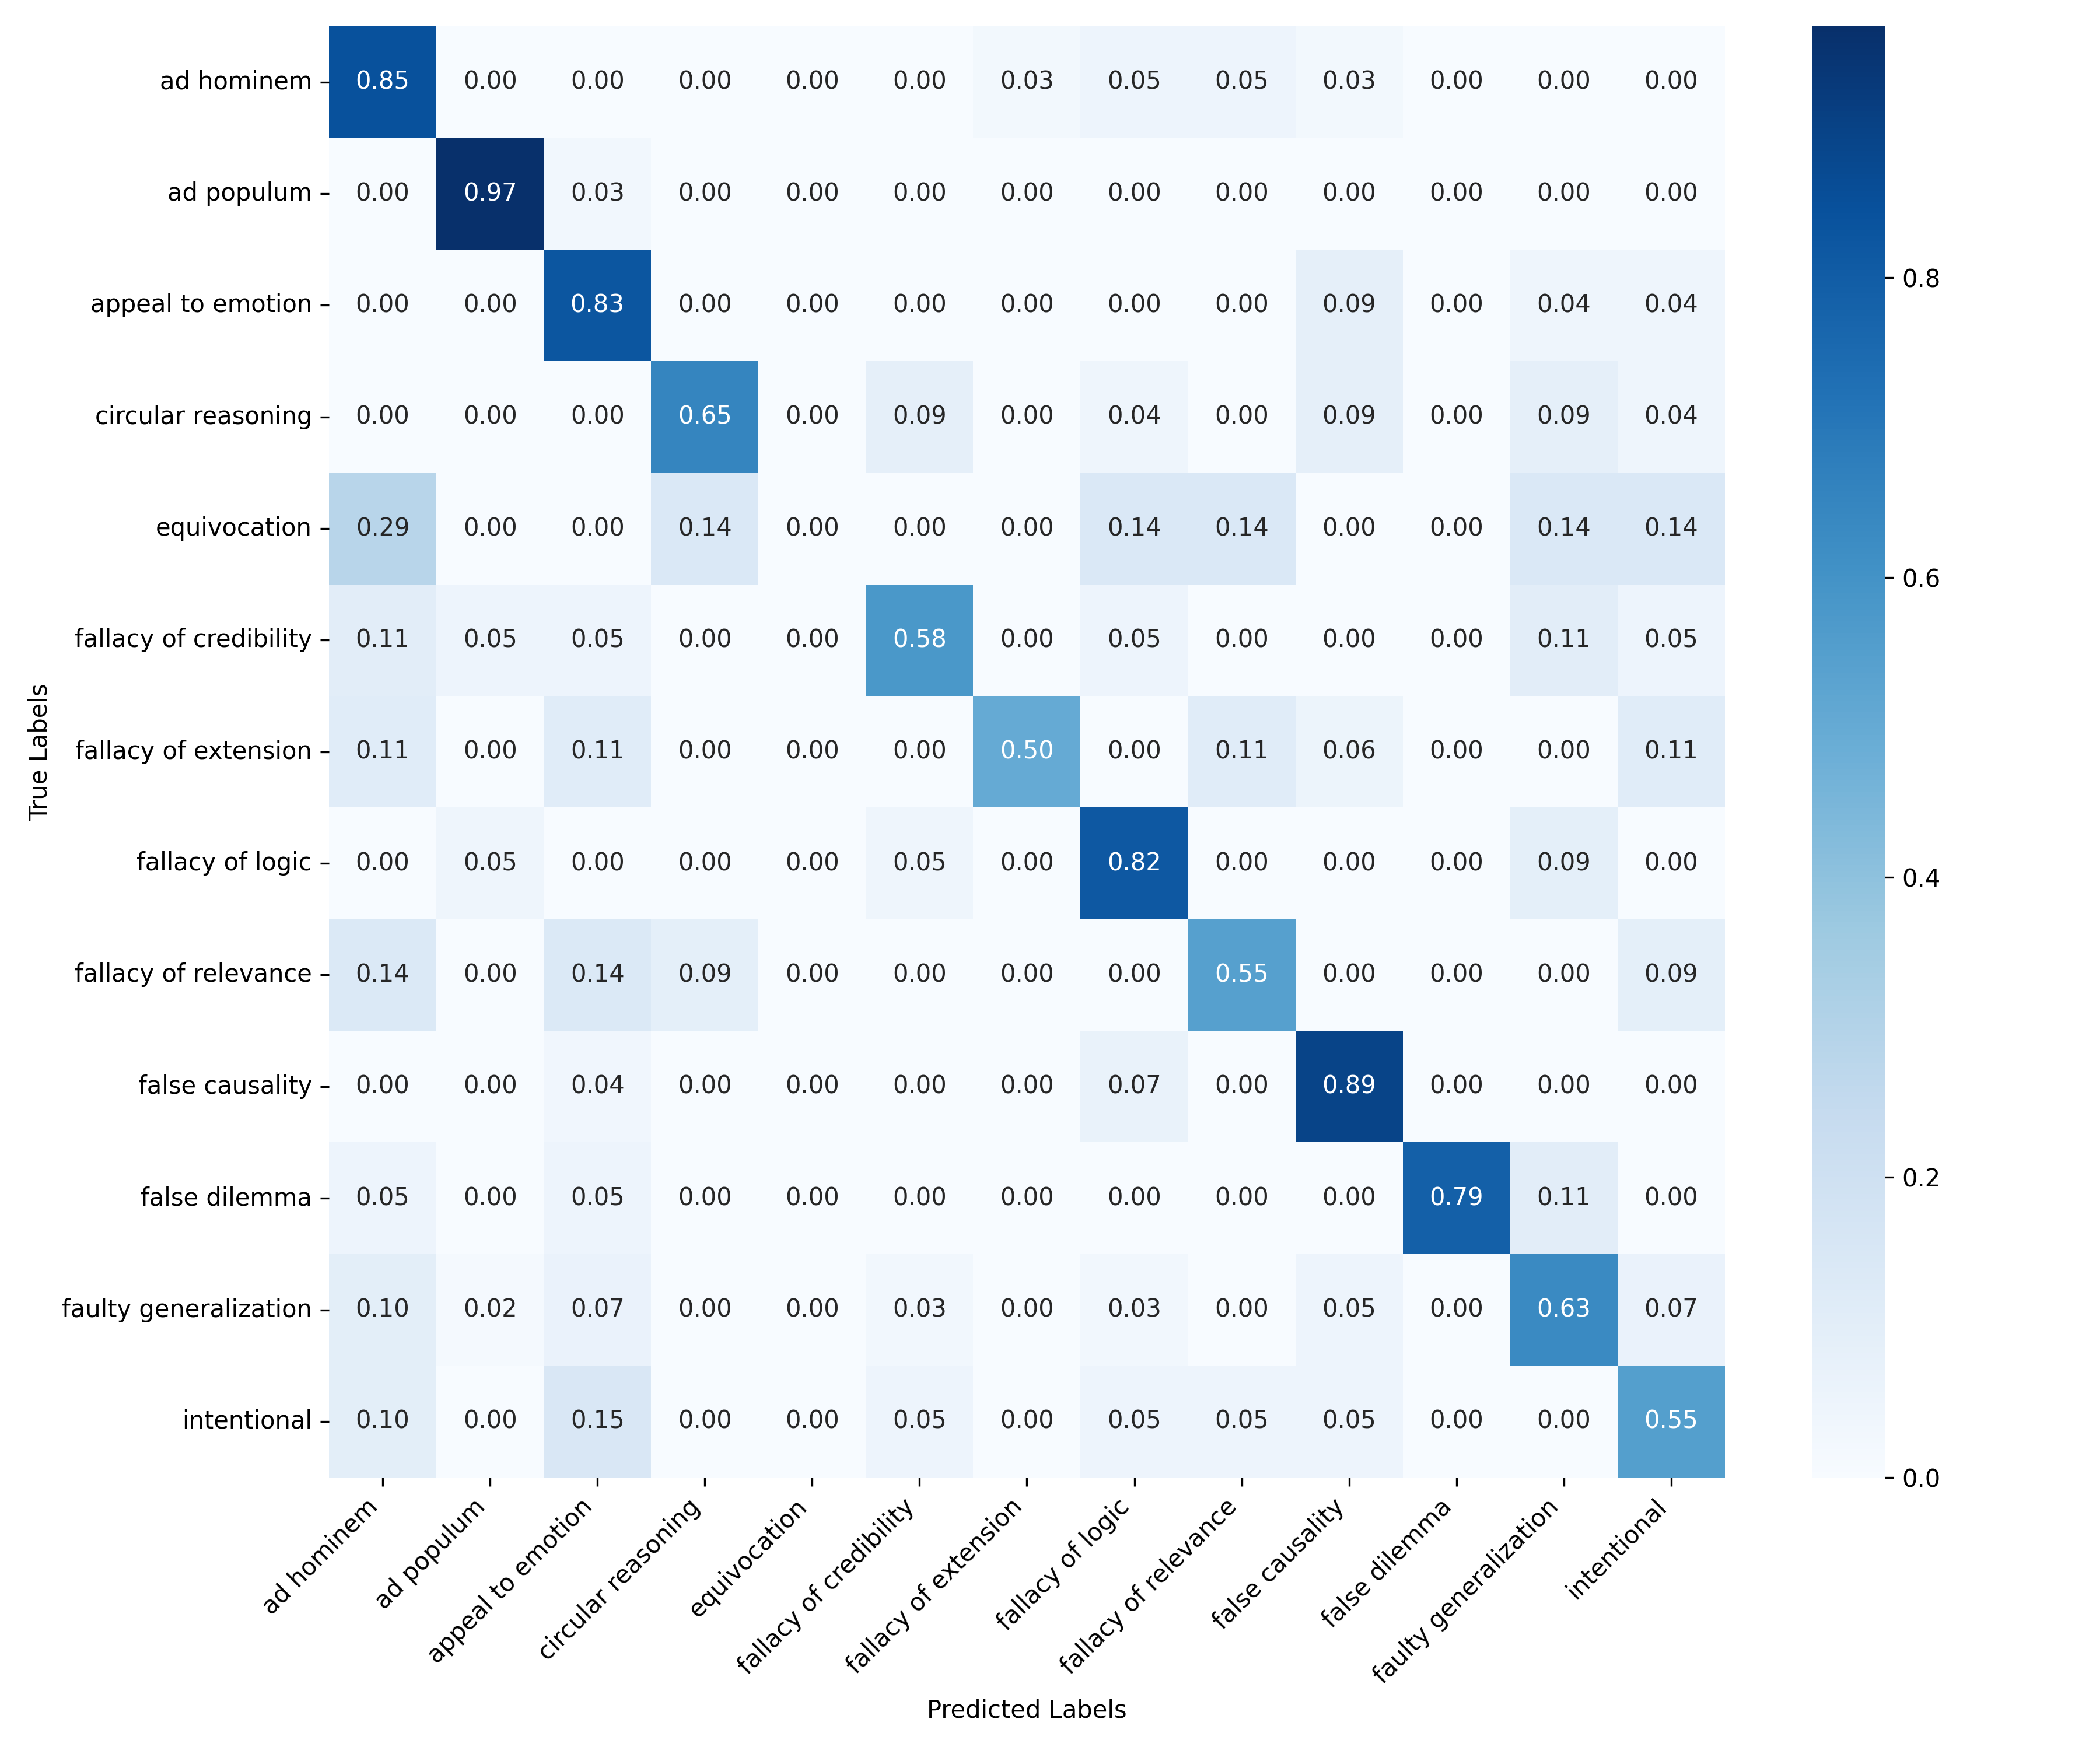
\includegraphics[width=\textwidth]{images/phi_logic_matrix.png}
        \caption{Phi-3.5-mini-instruct}
        \label{fig:phi_confusion}
    \end{subfigure}
    \caption{Performance of LLMS on LOGIC dataset for fallacy classification using a few-shot prompting approach. Each model's performance was visualized with a confusion matrix, providing insights into the classification accuracy across different fallacy types. The normalized confusion matrices for each model illustrate the proportion of correct and misclassified predictions for each fallacy class, allowing for a comparative analysis of model performance in detecting specific logical fallacies.}
    \label{fig:confusion_matrices_logic}
\end{figure*}

Figure~\ref{fig:confusion_matrices_logic} showed that Llama-3.2-3B-Instruct achieved balanced performance, excelling in ``ad populum'' (90\%) but face difficulties with complex fallacies. Qwen2.5-3B-Instruct demonstrated consistency in detecting straightforward fallacies, though it struggled with ``equivocation'' and ``fallacy of relevance''. Gemma-2-2b-it showed high accuracy in ``ad populum'' (84\%) and ``false causality'' (86\%) but found distinctions between emotional and relevance-based fallacies challenging. Similarly, Phi-3.5-mini-instruct performed well in identifying ``ad hominem'' (90\%), ``ad populum'' (97\%), and ``false causality'' (89\%) but struggled with fallacies like ``equivocation'' and ``intentional''. Overall, the models did well on fallacies that are easy to see, such ``ad populum'' and ``false causality,'' but they struggled with more subtle fallacies that need for interpretive reasoning, like ``equivocation'' and ``intentional''. 

\begin{figure*}[!ht]
    \centering
    \begin{subfigure}[b]{0.45\textwidth}
        \centering
        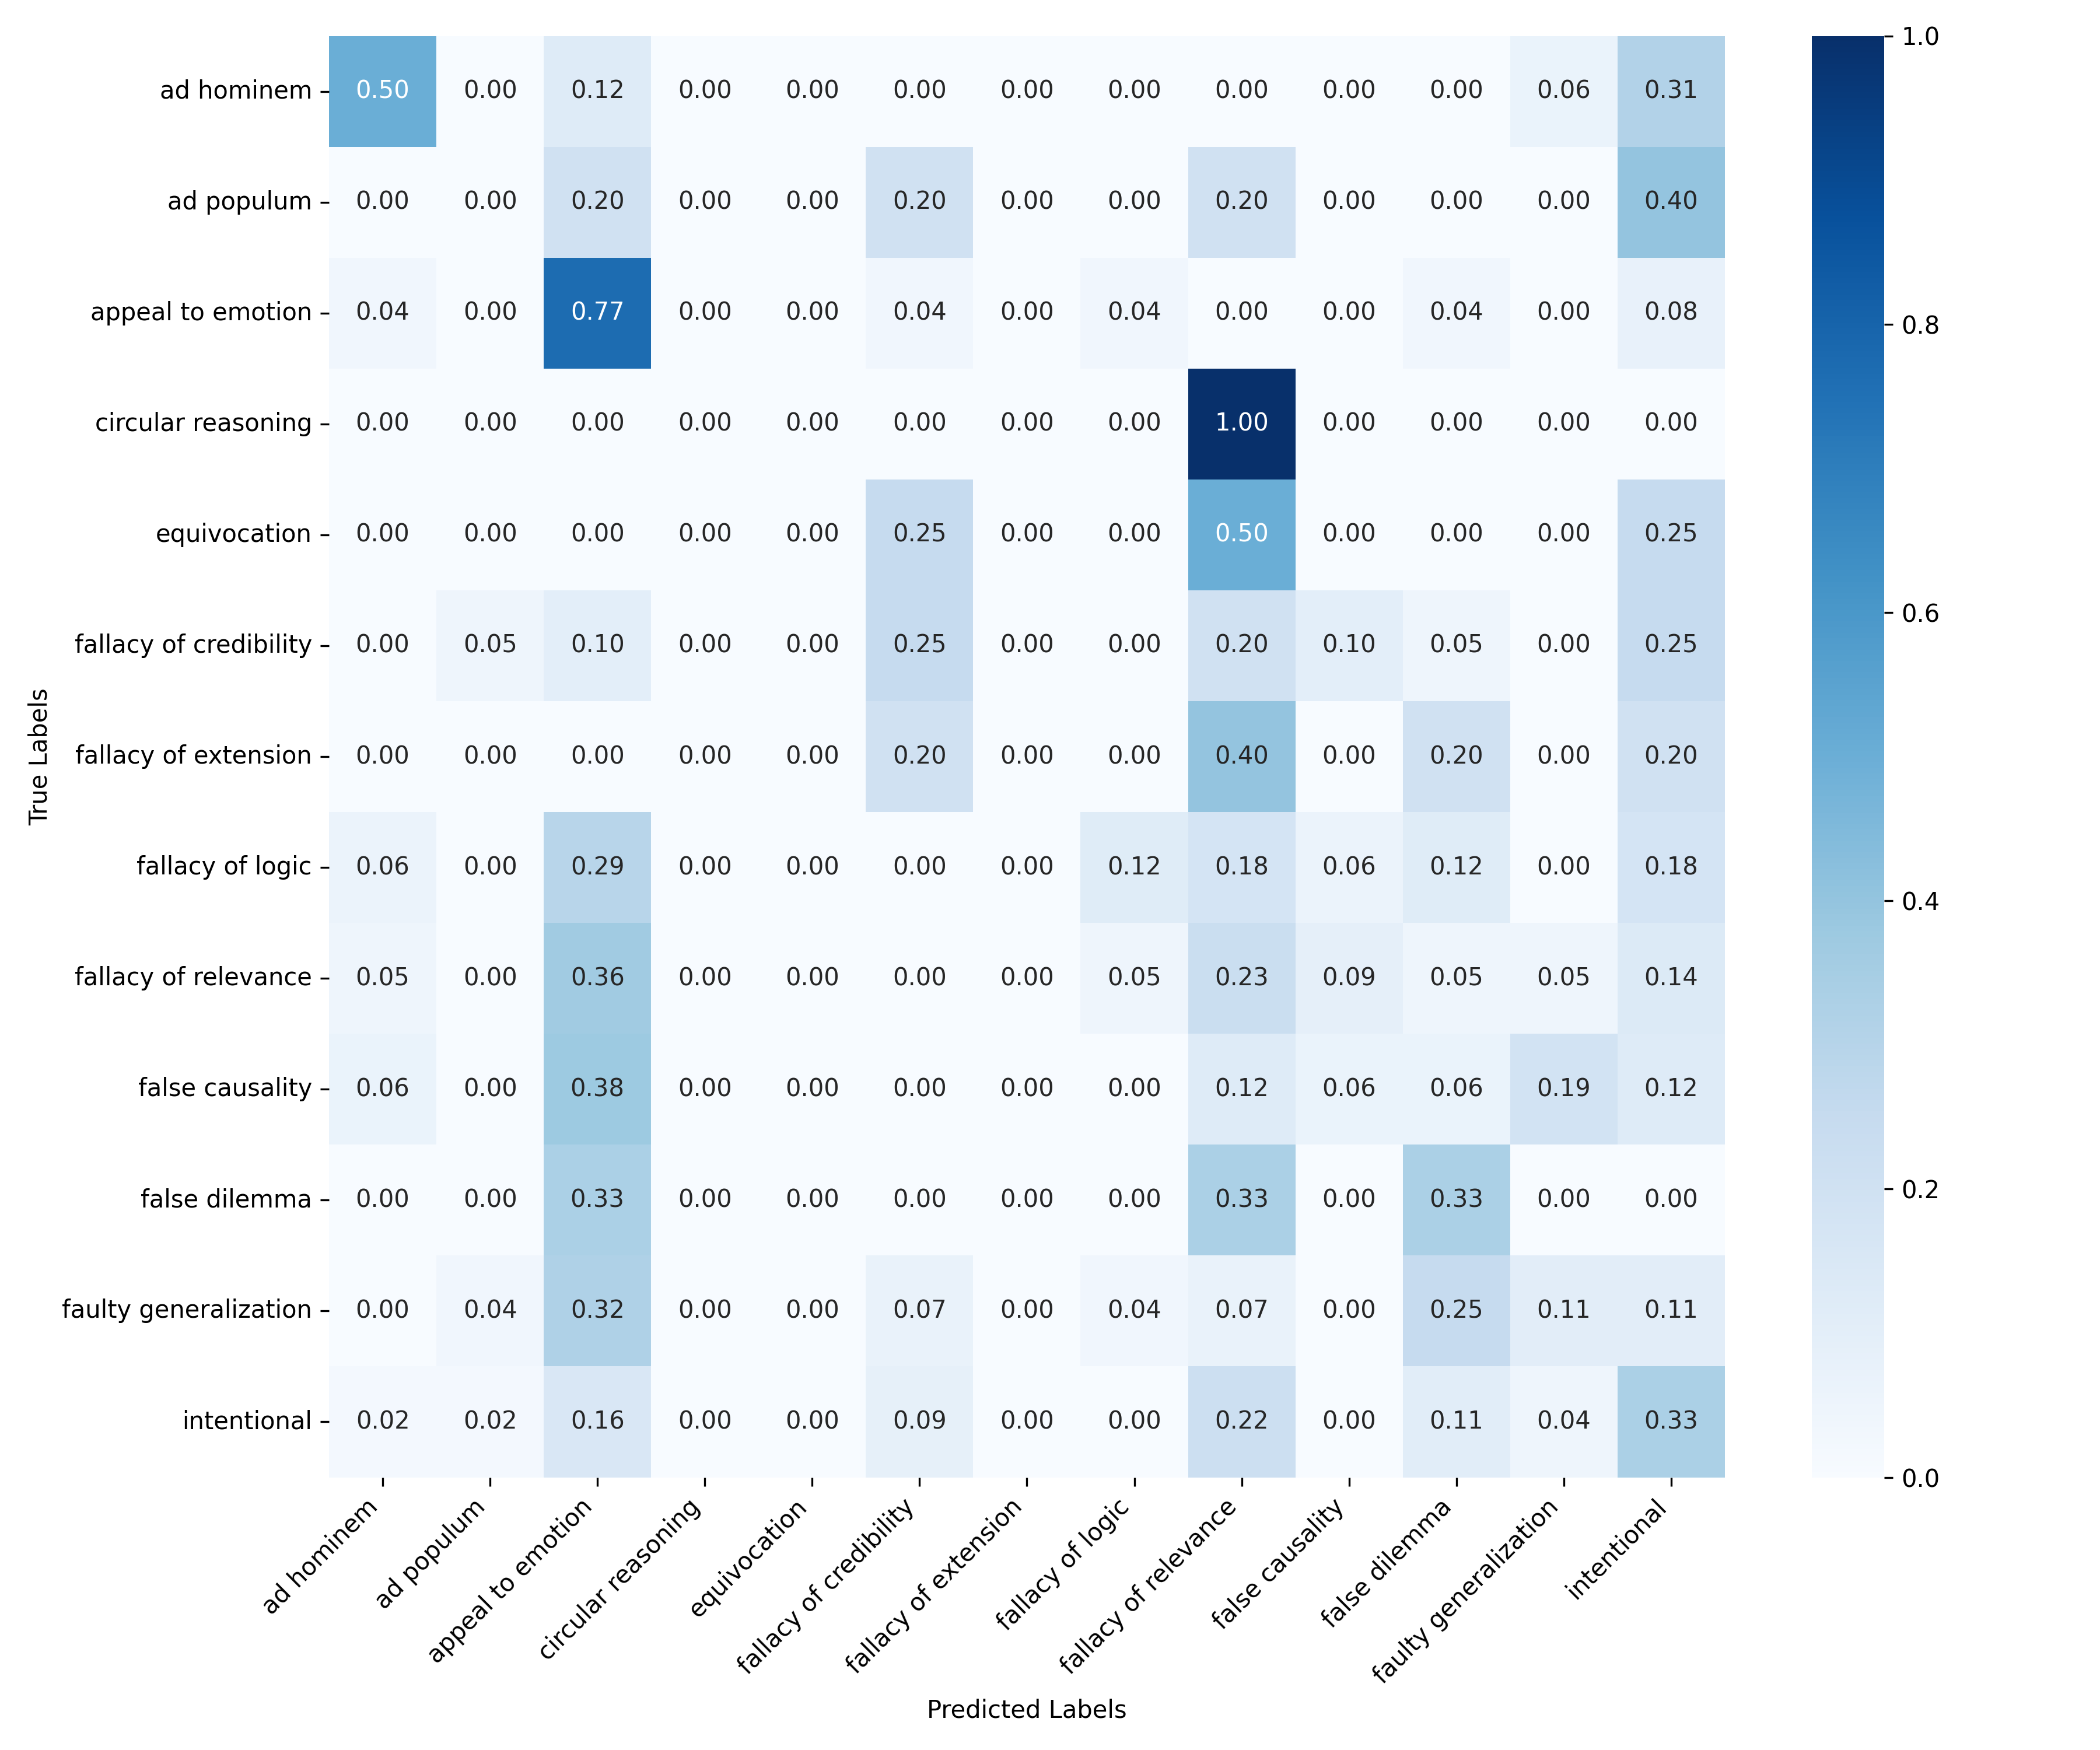
\includegraphics[width=\textwidth]{images/llama_climate_matrix.png}
        \caption{Llama-3.2-3B-Instruct}
        \label{fig:llama_confusion}
    \end{subfigure}
    \hfill
    \begin{subfigure}[b]{0.45\textwidth}
        \centering
        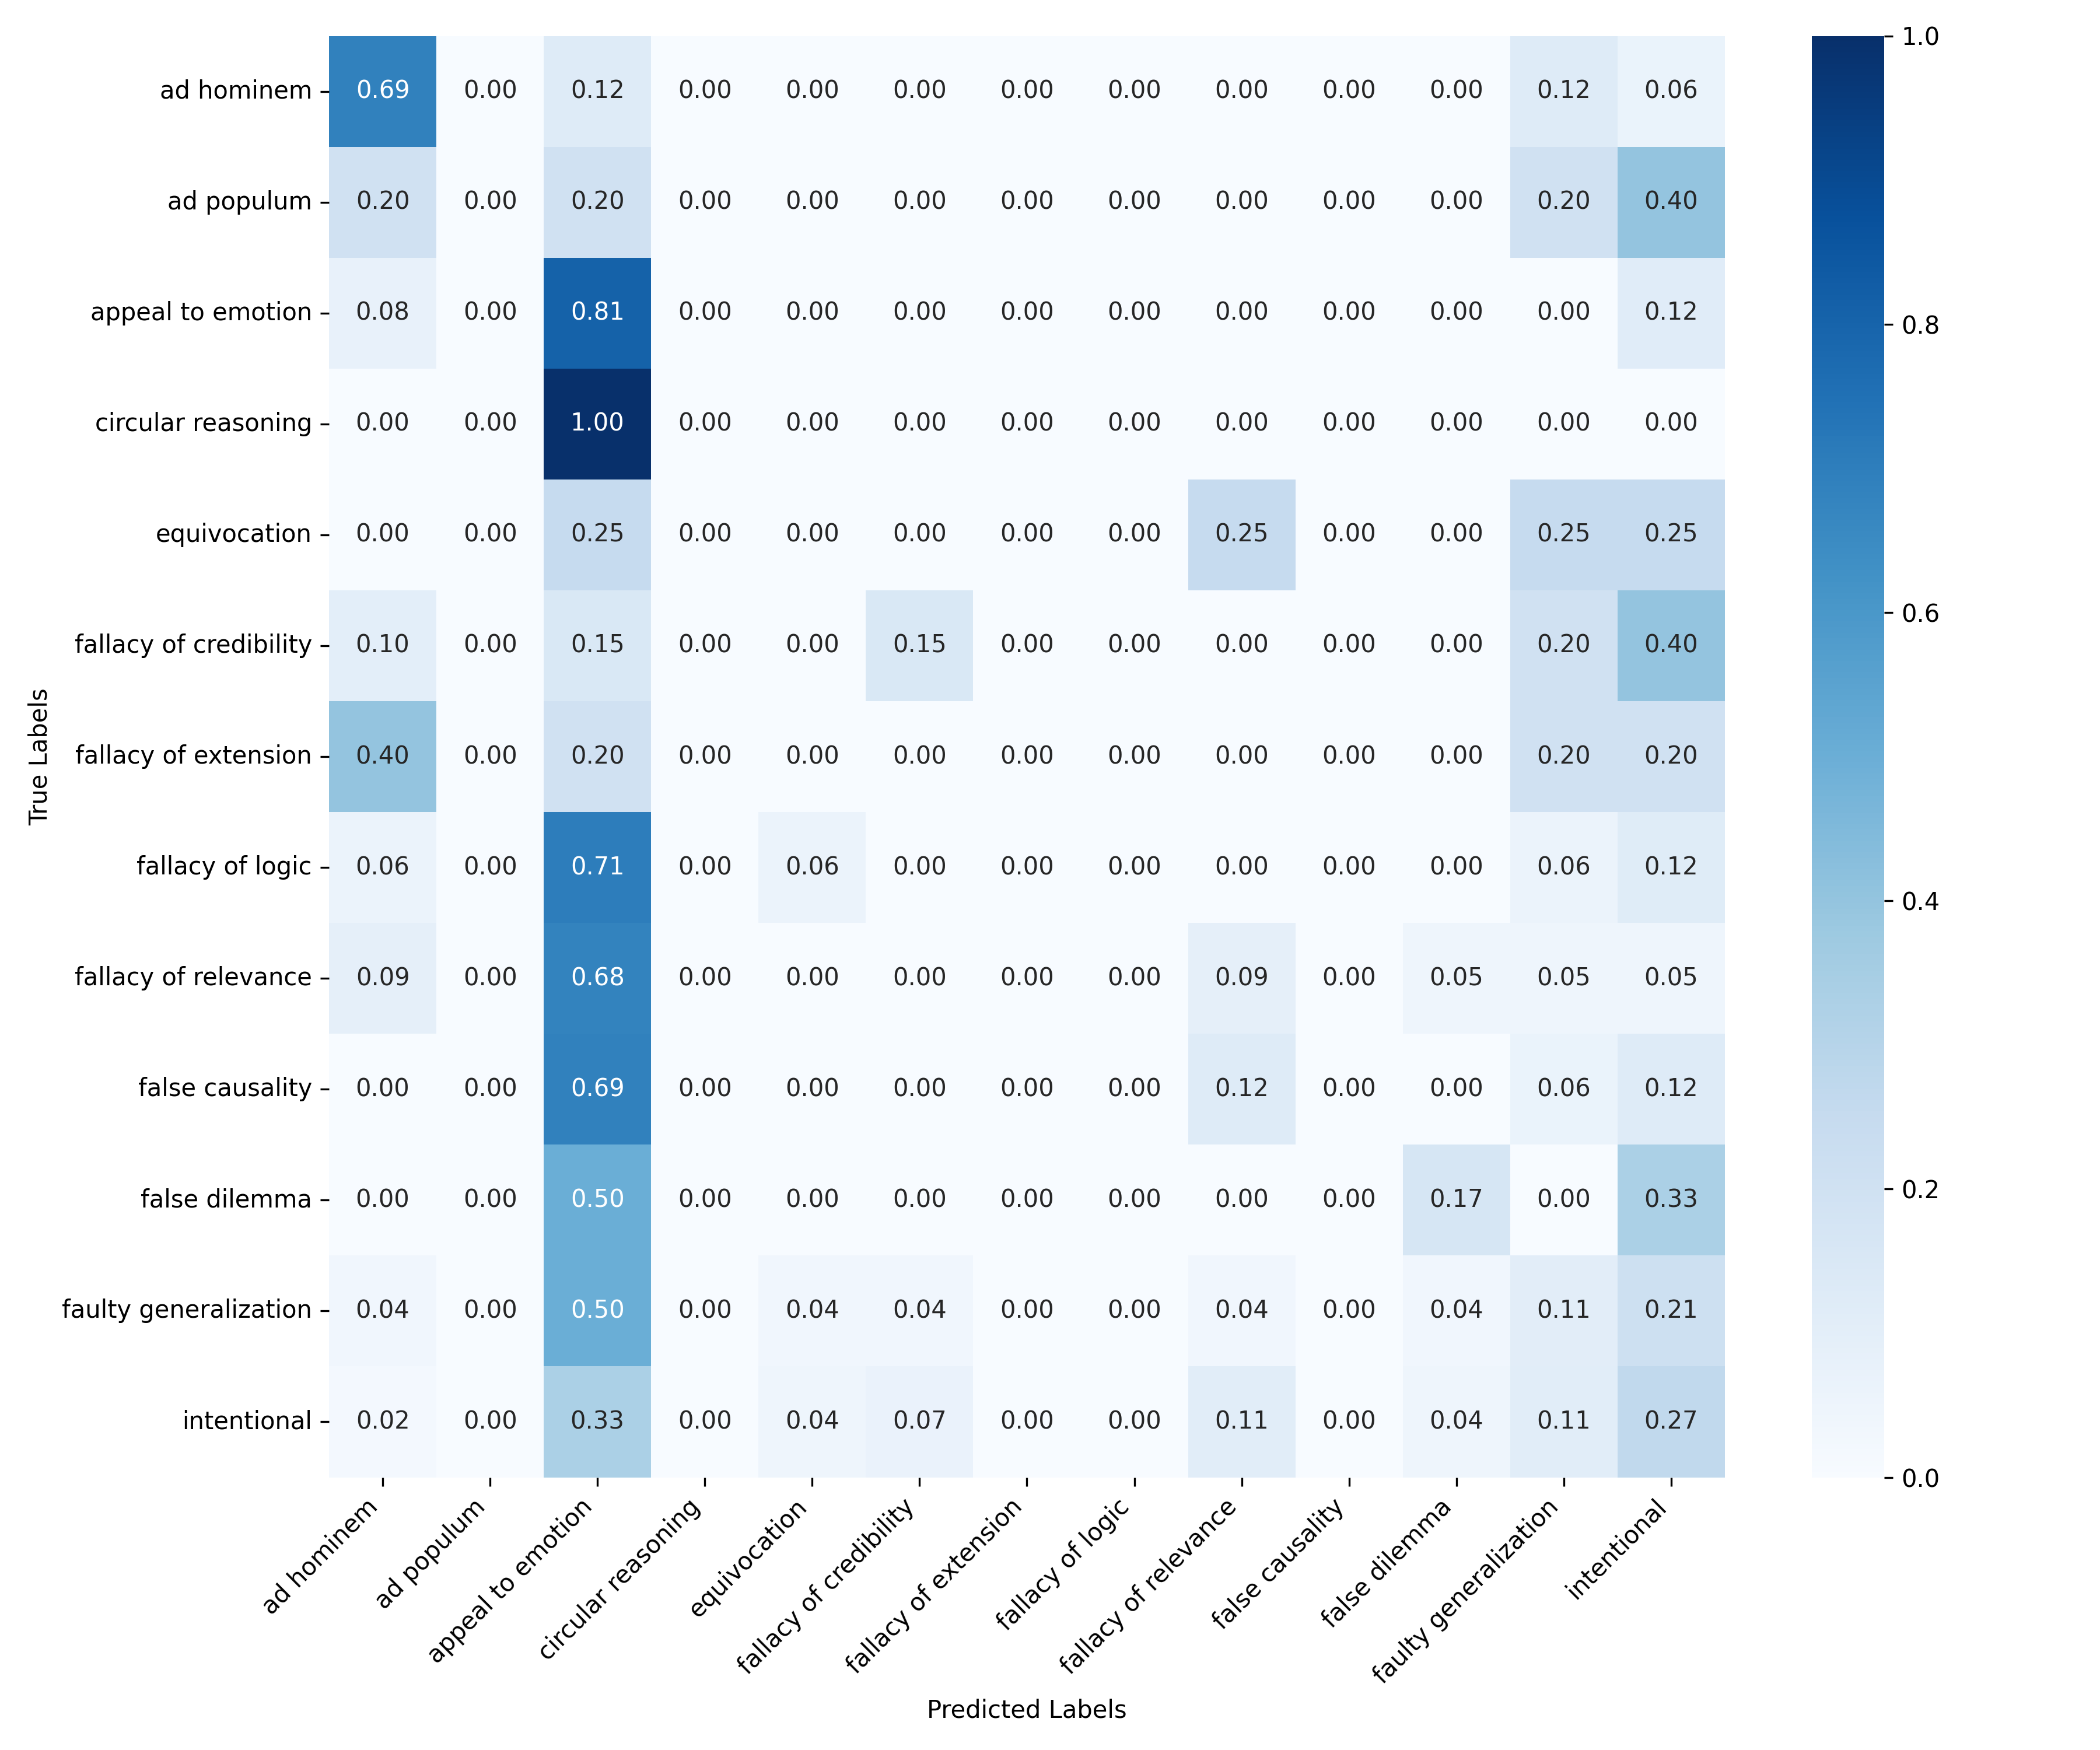
\includegraphics[width=\textwidth]{images/qwen_climate_matrix.png}
        \caption{Qwen2.5-3B-Instruct}
        \label{fig:qwen_confusion}
    \end{subfigure}
    \vskip\baselineskip
    \begin{subfigure}[b]{0.45\textwidth}
        \centering
        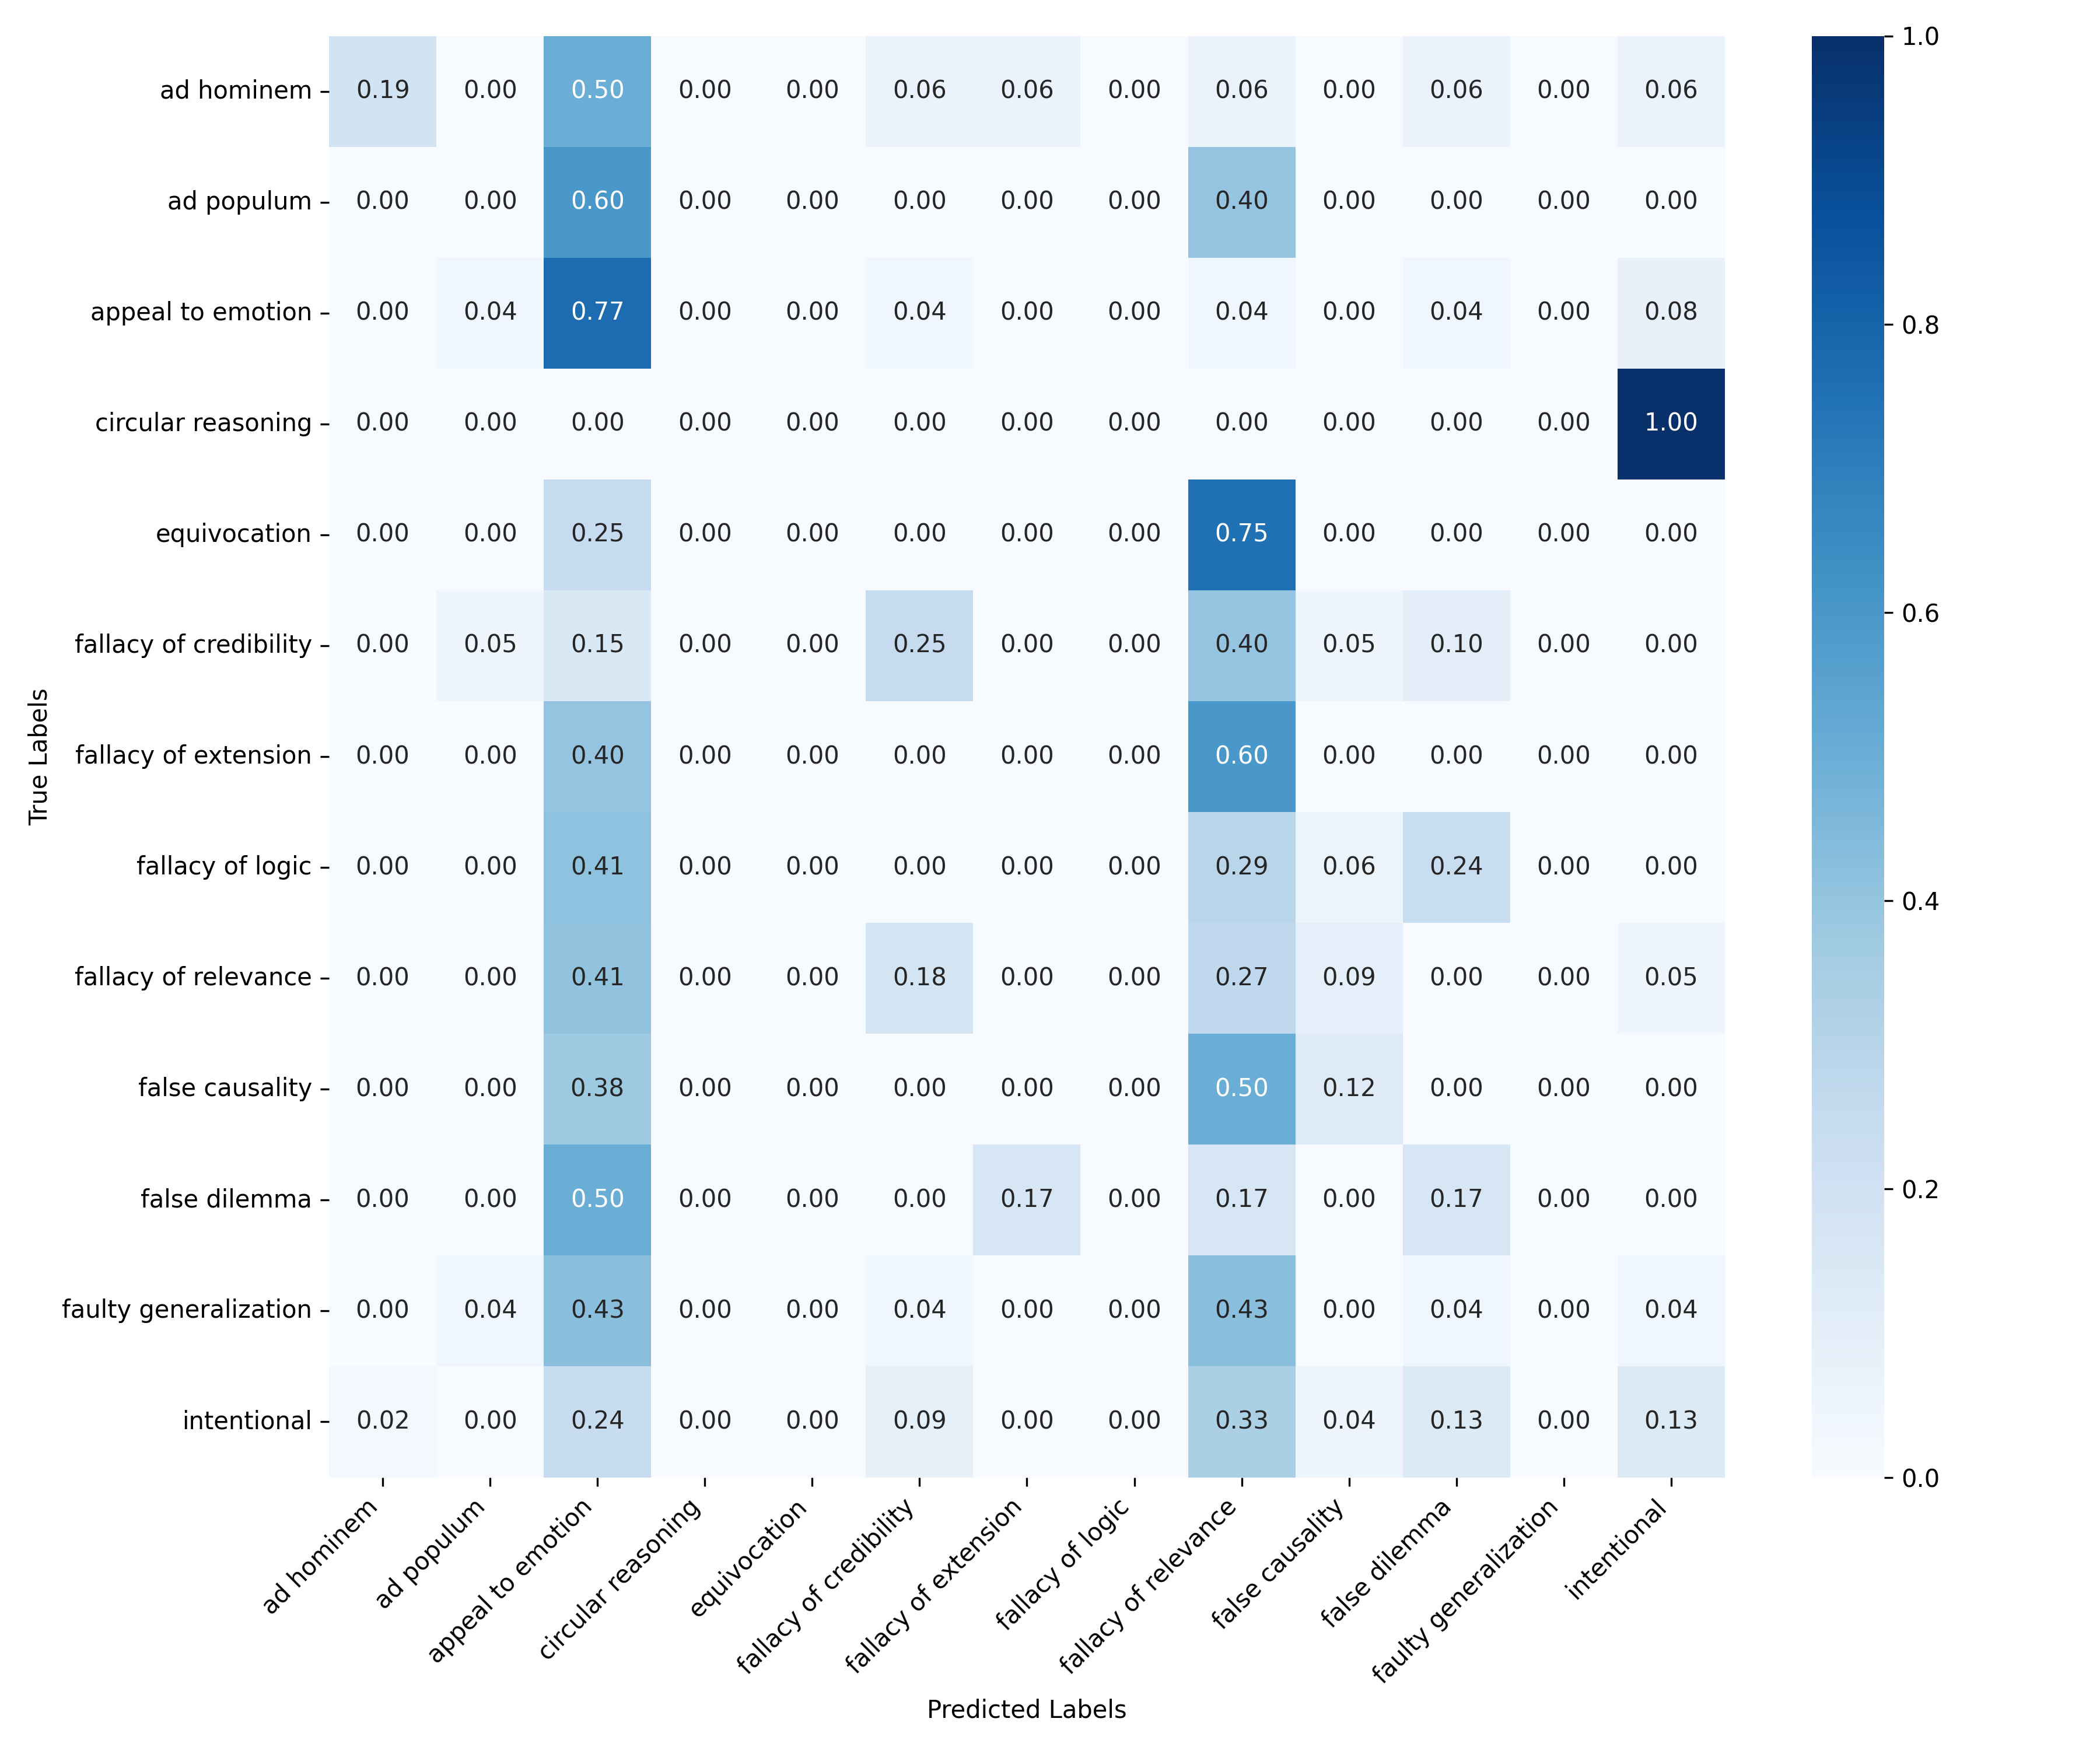
\includegraphics[width=\textwidth]{images/gemma_climate_matrix.png}
        \caption{Gemma-2-2b-it}
        \label{fig:gemma_confusion}
    \end{subfigure}
    \hfill
    \begin{subfigure}[b]{0.45\textwidth}
        \centering
        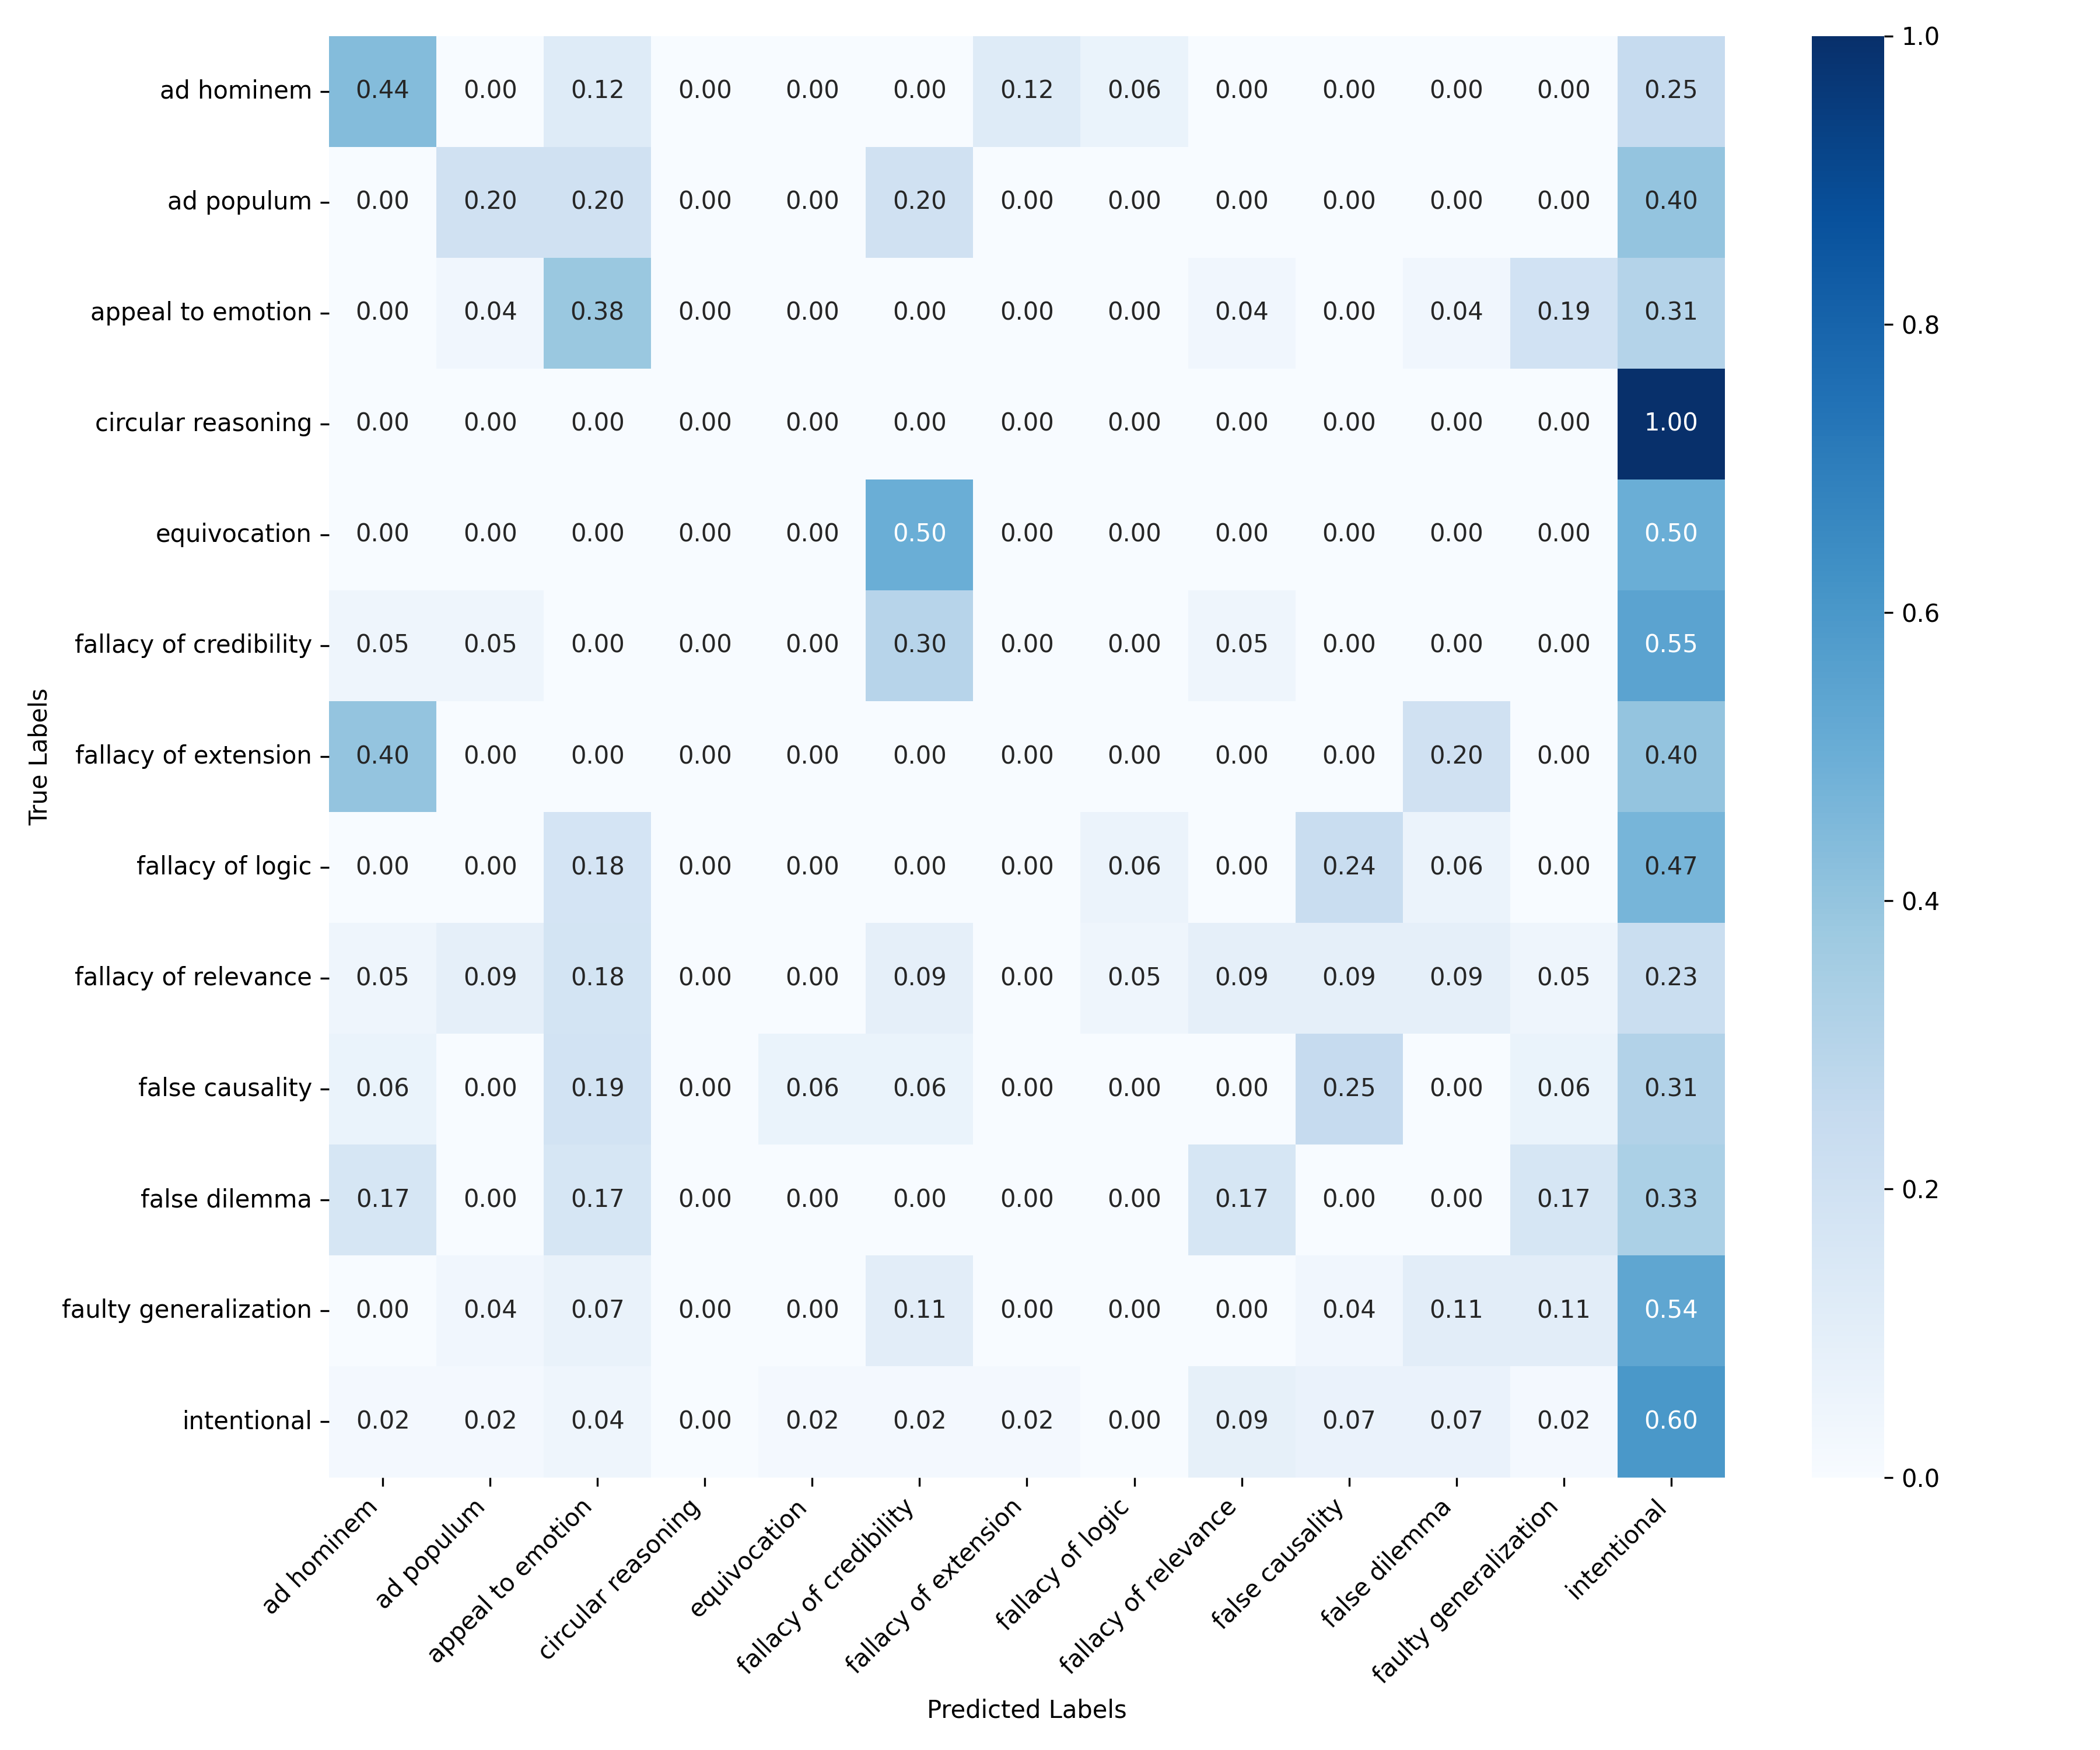
\includegraphics[width=\textwidth]{images/phi_climate_matrix.png}
        \caption{Phi-3.5-mini-instruct}
        \label{fig:phi_confusion}
    \end{subfigure}
    \caption{Performance of LLMs on LOGIC Climate dataset for fallacy classification using few-shot prompting. Each model’s performance was visualized through confusion matrices, providing insights into classification accuracy across different fallacy types. The results shed light on each model’s strengths and limitations in identifying specific climate-related fallacies.}
    \label{fig:confusion_matrices_climate}
\end{figure*}

Figure~\ref{fig:confusion_matrices_climate} showed that Llama-3.2-3B-Instruct did well on overt fallacies but struggled to differentiate between more subtle categories like ``fallacy of relevance.'' Similar to this, Qwen2.5-3B-Instruct demonstrated proficiency in ``appeal to emotion'' and ``circular reasoning,'' but mislabeled sophisticated fallacies such as ``fallacy of extension.'' Gemma-2-2b-it did well on ``equivocation'' and ``circular reasoning'' (75\%) but had trouble with fallacies that are closely linked, such as ``fallacy of relevance''. Phi-3.5-mini-instruct performed well in ``circular reasoning'' (100\%) but had trouble with more subtle fallacies like ``appeal to emotion'' and ``ad populum.'' Overall, all models shown limitations in interpretive reasoning by performing well at identifying ``circular reasoning'' but poorly at identifying subtle fallacies like ``equivocation'' and ``intentional''. Misclassifications that overlap, especially between ``ad hominem'' and ``appeal to emotion,'' show that linguistic similarities in climate-related fallacies pose a problem to LLMs.

\section{Discussion}
\subsection{Dataset} 
The majority of the examples in the datasets we used had one or two sentences, with the rare paragraph. However, real life usually consists of a few phrases or a few paragraphs. Although our analysis demonstrates that the LLMs functions for shorter texts. Lengthier texts—which are likely to contain a greater number of logical fallacies—may not yield the same results. To the best of our knowledge, there is no labeled dataset on logical fallacies for lengthy texts, thus generating one by hand would be necessary. Nevertheless, this would still warrant additional testing. 

\subsection{Prompt engineering}
Even though we designed a straightforward prompt to enhance the model’s few-shot learning capabilities and provide context when processing inputs, different
prompt constructions may impact the outcome. 

\subsection{Misclassifications}
The confusion matrices shed more light on the shortcomings of the models, especially when it comes to differentiating semantically related fallacies like appeal to emotion, circular reasoning, and fallacy of relevance. All models, regardless of size, exhibited confusion between these categories, highlighting the difficulty of detecting fallacies that share overlapping linguistic or argumentative features. This implies that existing models struggle with smaller distinctions, which probably led to the poorer recall scores seen in numerous models, even while they can handle fallacies with more distinguishing properties (like ad hominem and ad populum).

\section{Limitations}
First off, the datasets we used are mostly composed of brief text samples, usually consisting of just one or two phrases. Fallacies are frequently included into longer discourses, sometimes spanning several paragraphs, in real-world settings. As a result, it is unclear how well the models will perform on longer, more complicated texts. The thorough evaluation of model performance in such scenarios would require the creation of a labeled dataset with additional arguments. 

Second, the few-shot prompting strategy depends largely on prompt construction, even though it can be successful in some situations. The prompt's design has a big impact on the model's output, and different prompt formulations may provide different outcomes. Even though we followed a set pattern, trying out different prompt designs could result in even better results. Optimized prompt engineering methods should be investigated in future studies to improve model accuracy, especially for subtle fallacies.

Lastly, the models had trouble differentiating between fallacies that share semantic similarities, including ``appeal to emotion,'' ``circular reasoning,'' and ``fallacy of relevance.'' A shortcoming in the models' interpretive reasoning was highlighted by the numerous misclassifications caused by the overlapping linguistic and argumentation elements in these categories. These difficulties imply that in order to enhance their capacity to correctly distinguish closely similar logical fallacies, current LLMs could need more instruction or practice with a wider range of fallacy cases. Addressing these limitations can lead to advancing LLM capabilities for reliable logical fallacy detection in real-world applications.

\section{Conclusions and Future Work}
This study provides a comprehensive evaluation of several open source LLMs for detecting logical fallacies, using the LOGIC and LOGIC Climate datasets as benchmarks. We examined how well they performed in recognizing particular fallacy kinds using confusion matrices and common assessment metrics. According to our research, these models are effective at identifying simpler fallacies like ``circular reasoning,'' but they have trouble identifying more complex ones like ``equivocation'' and ``intentional,'' which call for more complex interpretive reasoning. The inability of current LLMs to handle subtle differences in logical arguments was highlighted by the frequent misclassifications caused by overlapping features among several fallacies. These findings imply that although LLMs may be useful for fallacy detection tasks, more work is necessary to ensure consistent accuracy, particularly in intricate, real-world texts. 

Future research should explore advanced prompt engineering and fine-tuning techniques to enhance LLMs’ interpretive capabilities. Furthermore, creating more extensive, contextually rich datasets may help give the models a stronger basis on which to detect errors in lengthy discourse. By resolving these issues, LLMs may develop into useful instruments for critical thinking exercises, enhancing the integrity and quality of information in a variety of fields, including media literacy, education, and automated content moderation. 

% \begin{table}
% \caption{Table captions should be placed above the
% tables.}\label{tab1}
% \begin{tabular}{|l|l|l|}
% \hline
% Heading level &  Example & Font size and style\\
% \hline
% Title (centered) &  {\Large\bfseries Lecture Notes} & 14 point, bold\\
% 1st-level heading &  {\large\bfseries 1 Introduction} & 12 point, bold\\
% 2nd-level heading & {\bfseries 2.1 Printing Area} & 10 point, bold\\
% 3rd-level heading & {\bfseries Run-in Heading in Bold.} Text follows & 10 point, bold\\
% 4th-level heading & {\itshape Lowest Level Heading.} Text follows & 10 point, italic\\
% \hline
% \end{tabular}
% \end{table}

% \noindent Displayed equations are centered and set on a separate
% line.
% \begin{equation}
% x + y = z
% \end{equation}
% Please try to avoid rasterized images for line-art diagrams and
% schemas. Whenever possible, use vector graphics instead (see
% Fig.~\ref{fig1}).

% \begin{figure}
% 
\includegraphics[width=\textwidth]{fig1.eps}
% \caption{A figure caption is always placed below the illustration.
% Please note that short captions are centered, while long ones are
% justified by the macro package automatically.} \label{fig1}
% \end{figure}

% \begin{theorem}
% This is a sample theorem. The run-in heading is set in bold, while
% the following text appears in italics. Definitions, lemmas,
% propositions, and corollaries are styled the same way.
% \end{theorem}

% the environments 'definition', 'lemma', 'proposition', 'corollary',
% 'remark', and 'example' are defined in the LLNCS documentclass as well.

% \begin{proof}
% Proofs, examples, and remarks have the initial word in italics,
% while the following text appears in normal font.
% \end{proof}
% For citations of references, we prefer the use of square brackets
% and consecutive numbers. Citations using labels or the author/year
% convention are also acceptable. The following bibliography provides
% a sample reference list with entries for journal
% articles~\cite{ref_article1}, an LNCS chapter~\cite{ref_lncs1}, a
% book~\cite{ref_book1}, proceedings without editors~\cite{ref_proc1},
% and a homepage~\cite{ref_url1}. Multiple citations are grouped
%~\cite{ref_article1,ref_lncs1,ref_book1},
%~\cite{ref_article1,ref_book1,ref_proc1,ref_url1}.

\begin{credits}

\subsubsection{\discintname}
The authors have no competing interests to declare that are
relevant to the content of this article.
\end{credits}
%
% ---- Bibliography ----
%
% BibTeX users should specify bibliography style 'splncs04'.
% References will then be sorted and formatted in the correct style.
%

\bibliographystyle{splncs04} % We choose the ``plain'' reference style
\bibliography{refs} % Entries are in the refs.bib file


\end{document}
